% DRIVER DE PREVISUALIZACIÓN GLOBAL (no forma parte de la entrega).
% Junta en un solo PDF TODO lo redactado de la memoria, con portada oficial,
% índice y bibliografía. Usa natbib+bibtex (ieeetr) en lugar de biblatex+biber
% porque biber no está instalado. El documento final usa tfg_etsiinf_JuanLlorens.tex.
\documentclass[a4paper,11pt]{book}
\usepackage[T1]{fontenc}
\usepackage[utf8]{inputenc}
\usepackage[english]{babel} % preview: spanish.ldf no está instalado; nombres forzados abajo
\usepackage{lmodern}
\usepackage{amsmath}
\usepackage[top=3.5cm,bottom=3.5cm,right=3cm,left=3cm]{geometry}
\usepackage{booktabs}
\usepackage{longtable}
\usepackage{multirow}
\usepackage{graphicx}
\graphicspath{{figuras/}{../../figures/}}
\usepackage{float}
\usepackage{tikz}
\usepackage{xcolor}
\usepackage{parskip}
\usepackage[numbers]{natbib}
\usepackage{hyperref}

%% Tipo de estudios
\newcommand{\Estudios}{Grado}

%% Título de los estudios (pendiente de confirmar según plan: 10ML / 10ID-II / 10II)
\newcommand{\TituloEstudios}{Matem\'aticas e Inform\'atica}

%% Departamento de la Tutora
\newcommand{\Departamento}{Departamento de Lenguajes y Sistemas Inform\'aticos}

%% Nombre y apellidos del autor
\newcommand{\NombreAutor}{Juan Llorens Mart\'inez}

%% Nombre y apellidos de la Tutora
\newcommand{\NombreTutor}{Adriana Toni Delgado}

%% Título del Trabajo
\newcommand{\TituloTFG}{Predicci\'on de Desplazamientos de Aves mediante Modelos Probabil\'isticos y Machine Learning: Un Enfoque H\'ibrido}

%% Fecha de lectura (mes año)
\newcommand{\Fecha}{julio 2026}

% Establecer los datos con los comandos estándares de LaTeX
\title{\TituloTFG}
\author{\NombreAutor}
\date{\Fecha}


\begin{document}
% Este TeXLive no tiene babel-spanish (falta spanish.ldf): forzamos los nombres
% en castellano SOLO en el preview. En una instalación completa babel ya lo hace solo.
\renewcommand{\chaptername}{Capítulo}
\renewcommand{\figurename}{Figura}
\renewcommand{\tablename}{Tabla}
\renewcommand{\contentsname}{Tabla de contenidos}
\renewcommand{\bibname}{Bibliografía}

\input{portada/portada}
\tableofcontents

\chapter*{Resumen}

La proliferación de los dispositivos de geolocalización ha transformado el estudio
del movimiento animal: el cuello de botella de la disciplina se ha desplazado de
registrar dónde ha estado un animal a anticipar dónde estará. Este trabajo aborda
esa pregunta sobre una especie concreta, la gaviota sombría (\textit{Larus fuscus}),
un migrante de larga distancia cuyo corredor une las zonas de cría del norte de
Europa con las áreas de invernada del este de África, a partir de datos públicos de
seguimiento GPS. El problema se plantea a escala diaria: dada la posición de un
individuo hoy, predecir dónde estará mañana.

Para ello se diseña y evalúa un enfoque híbrido que combina modelos probabilísticos
y aprendizaje automático. A partir de los registros GPS en bruto se construye una
secuencia diaria homogénea de posiciones por individuo, con los huecos del
seguimiento representados de forma explícita, que sirve de base común a todos los
modelos. Sobre ella se articulan tres piezas. Una cadena de Markov visible establece
una baseline interpretable y fija el criterio de evaluación común, frente a la
referencia trivial de suponer que el animal permanecerá donde está. Un modelo oculto
de Markov infiere, sin supervisión, el régimen de comportamiento de cada día
(estacionario o en migración) y se valida por su coherencia con la fenología de la
especie. Ese régimen alimenta, como una variable más, a modelos de aprendizaje
supervisado (Random Forest, XGBoost y LightGBM), que predicen el desplazamiento
empleando únicamente información disponible antes del instante que se predice. Por
último, una herramienta de cartografía interactiva permite visualizar y comparar
sobre el mapa las predicciones de los distintos modelos.

El enfoque aporta en tres frentes complementarios. Calibra la incertidumbre de cada
predicción mediante una banda que la herramienta interactiva traslada al mapa; aísla
el régimen de migración, que es donde anticipar el desplazamiento resulta
verdaderamente informativo, frente a los largos periodos estacionarios propios de la
especie; y caracteriza con datos el techo estructural que impone predecir a un día con
información puramente local, un límite inherente al horizonte del problema más que a un
modelo concreto. La formulación del problema como regresión de cuantiles es la que
mejor concilia la precisión de la posición estimada con una incertidumbre bien
calibrada.

La contribución del trabajo es triple: la caracterización rigurosa de un límite
estructural de la predicción a corto plazo, una herramienta interactiva para comparar
modelos sobre el territorio, y un criterio metodológico transversal, el de exigir
coherencia biológica a todo resultado antes de darlo por válido. De ahí se derivan las
líneas de trabajo futuro, que apuntan a modelos de secuencia, a la incorporación del
viento y a la predicción a varios pasos.

\begin{otherlanguage}{english}
  \chapter*{Abstract}

  \todo[inline]{Abstract of the Final Degree Project. Maximum length: 2 pages.}
\end{otherlanguage}


%%%%%%%%%%%%%%%%%%%%%%%%%%%%%%%%%%%%%%%%%%%%%%%%%%%%%%%%%%%
%% Final del resumen.
%%%%%%%%%%%%%%%%%%%%%%%%%%%%%%%%%%%%%%%%%%%%%%%%%%%%%%%%%%%

\chapter{Introducción}
\label{ch:intro}

\section{Motivación}
\label{sec:intro-motivacion}

La generalización de los dispositivos de geolocalización ha transformado el
estudio del movimiento animal \cite{kays2015}. Repositorios como Movebank acumulan
hoy millones de posiciones GPS de miles de individuos, de modo que el cuello de
botella de la
disciplina se ha desplazado de \emph{registrar} dónde ha estado un animal a
\emph{modelar y anticipar} dónde estará. Predecir la posición futura a partir del
rastro histórico es, sin embargo, un problema abierto: el movimiento combina
rutina y cambio, responde a factores ambientales y varía de un individuo a otro.
Esa dificultad motiva combinar modelos probabilísticos y técnicas de aprendizaje
automático en un enfoque híbrido, en lugar de depender de un único tipo de
modelo.

Este trabajo aborda esa pregunta sobre una especie concreta, la gaviota sombría
(\textit{Larus fuscus}), un migrante de larga distancia cuyo corredor se extiende
entre las zonas de cría del norte de Europa y las áreas de invernada del este de
África. Su ciclo anual está marcado por una fenología nítida (cría en junio y
julio, paso migratorio en primavera y otoño e invernada en los meses centrales
del invierno), lo que la convierte en un caso idóneo: una única especie, con un
patrón estacional fuerte y datos de seguimiento GPS públicos
\cite{movebank_gulls, wikelski2015}. El conjunto de datos concreto se describe en
el capítulo \ref{ch:o1}.

\section{Definición del problema y enfoque híbrido}
\label{sec:intro-enfoque}

La pregunta que vertebra el trabajo es deliberadamente simple: dada la posición
de un individuo hoy, ¿dónde estará mañana? Se trata de una predicción a un día
sobre una secuencia de posiciones diarias, la que produce la preparación de los
datos del capítulo \ref{ch:o1}. Plantearla a esa escala (un paso por día) evita
depender de la frecuencia irregular del seguimiento GPS y centra el problema en
el desplazamiento, no en el muestreo.

Predecir ese desplazamiento es difícil porque el movimiento alterna regímenes muy
distintos (días casi inmóviles y días de migración de cientos de kilómetros) y
porque cada ave sigue su propia ruta, de modo que un patrón
aprendido de la población no describe sin más a un individuo concreto. A ello se
añade una tensión metodológica: los modelos probabilísticos clásicos son
interpretables pero limitados, mientras que el aprendizaje automático capta
relaciones no lineales a costa de transparencia. El enfoque híbrido de este
trabajo combina dos piezas para afrontarla: una baseline probabilística
interpretable, frente a la que se mide todo lo demás, y un predictor que une un
modelo de comportamiento con aprendizaje automático para tratar de superarla
(figura \ref{fig:intro-hibrido}).

\begin{figure}[H]
  \centering
  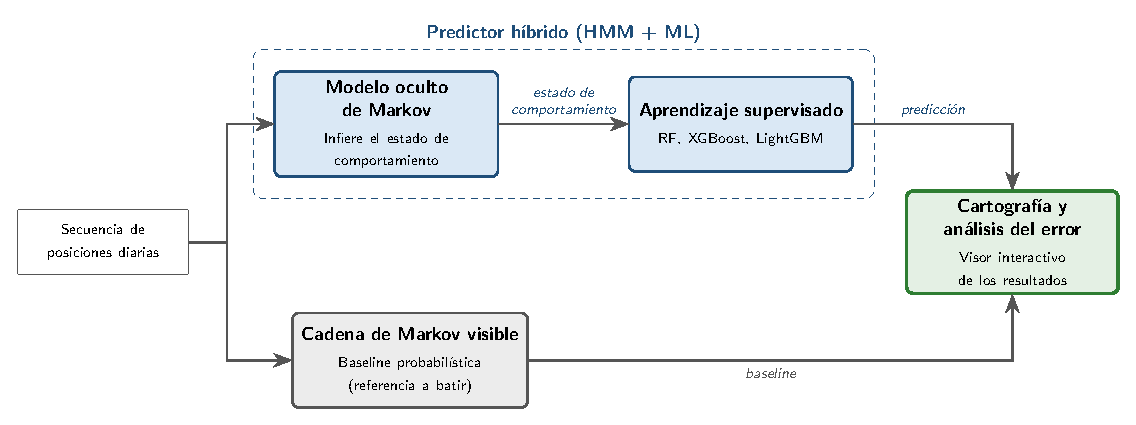
\includegraphics[width=\linewidth]{intro_enfoque_hibrido.pdf}
  \caption[El enfoque híbrido: baseline frente a predictor combinado]{Esquema del
  enfoque híbrido. A partir de la secuencia de posiciones diarias, la cadena de
  Markov visible (vía inferior) actúa como baseline y el predictor híbrido (vía
  superior) combina el modelo oculto de Markov con el aprendizaje supervisado;
  ambas vías se comparan en el visor interactivo de la posición y el error.}
  \label{fig:intro-hibrido}
\end{figure}

La baseline es una cadena de Markov visible, que estima la posición del día
siguiente a partir de la celda actual; es interpretable y fija el criterio de
comparación común al resto de modelos. El predictor híbrido, por su parte,
encadena dos modelos: un modelo oculto de Markov infiere para cada día un estado
de comportamiento no observado (estacionario o en migración), y ese estado alimenta,
como una variable más, a los modelos de aprendizaje supervisado (Random Forest,
XGBoost y LightGBM), que predicen el desplazamiento incorporando además variables
propias de cada individuo. Esa unión de un modelo probabilístico de comportamiento
con el aprendizaje automático es lo que da al enfoque su carácter híbrido y lo que
busca superar a la baseline. Para interpretar los resultados se desarrolla además
una herramienta de cartografía interactiva, que permite visualizar de un vistazo
sobre el mapa las predicciones de los modelos y analizar dónde y cuándo acierta o
falla cada una.

Conviene anticipar el hallazgo que recorre todos los capítulos: la regla trivial
de suponer que mañana el ave seguirá donde está hoy (la persistencia) resulta
sorprendentemente difícil de superar, porque la especie pasa la mayor parte de
los días sin cambiar de lugar. El valor del trabajo no reside, por tanto, en un
salto de exactitud sobre esa regla, sino en calibrar mejor la incertidumbre, en
aislar el régimen de migración (donde la predicción sí aporta) y en caracterizar
el techo estructural de predecir a un día con información local.

\section{Objetivos del trabajo}
\label{sec:intro-objetivos}

El objetivo general del trabajo es diseñar y evaluar un enfoque híbrido, que
combine modelos probabilísticos y aprendizaje supervisado, para predecir el
desplazamiento diario de la gaviota sombría a partir de datos de seguimiento GPS.
Reviste especial interés la comparación sistemática de las distintas soluciones
desarrolladas, medidas todas con una métrica probabilística común y frente a
baselines explícitas.

Este objetivo general se concreta en cinco objetivos específicos:

\begin{enumerate}
  \item Transformar los registros GPS en bruto en una secuencia diaria homogénea
  por individuo, con los huecos del seguimiento representados de forma explícita,
  que sirva de base común a todos los modelos.
  \item Establecer una baseline predictiva interpretable mediante cadenas de
  Markov visibles, y fijar con ella el criterio de evaluación (el log-loss) y la
  referencia de persistencia frente a la que se contrasta el resto de modelos.
  \item Detectar el régimen de comportamiento de cada día (estacionario o en
  migración) mediante un modelo oculto de Markov, comprobando que los estados
  inferidos son coherentes con la fenología de la especie.
  \item Predecir la posición del día siguiente con modelos de aprendizaje
  supervisado (Random Forest, XGBoost y LightGBM) que integran el comportamiento
  inferido y variables propias de cada individuo, empleando solo información
  disponible antes del instante que se predice.
  \item Desarrollar una herramienta de cartografía interactiva que permita
  visualizar y comparar sobre el mapa los resultados de los modelos.
\end{enumerate}

\chapter{Preliminares}
\label{ch:preliminares}

Este capítulo reúne el contexto en la literatura y los fundamentos teóricos sobre
los que se apoya el trabajo. Su propósito es servir de referencia: los capítulos
de desarrollo emplean estas herramientas en su forma aplicada y remiten aquí, en
lugar de reexplicarlas. Se presenta cada familia de modelos junto con el papel que
desempeña en el problema, y se reserva para los capítulos correspondientes la
justificación de las decisiones concretas (tamaño de celda, número de estados,
hiperparámetros) y la definición de las métricas de evaluación.

\section{El análisis y la predicción del movimiento animal}
\label{sec:prelim-movimiento}

El movimiento es uno de los procesos que articulan la vida de un animal, pues
conecta su fisiología y su comportamiento con el entorno en el que habita. La
ecología del movimiento propone un marco unificador para estudiarlo, que sitúa el
desplazamiento de un organismo en el centro y lo relaciona con su estado interno,
sus capacidades de navegación y locomoción y los factores externos que lo
condicionan \cite{nathan2008}. La generalización de los dispositivos de
geolocalización ha convertido esta disciplina en un campo intensivo en datos:
repositorios como Movebank acumulan grandes volúmenes de trayectorias y han
abierto el análisis del movimiento a las técnicas estadísticas y computacionales
\cite{kays2015, demsar2015}.

Con esa abundancia de datos, el interés se desplaza de describir trayectorias
pasadas a modelarlas y anticipar posiciones futuras. Esa predicción exige combinar
herramientas de naturaleza distinta, en lugar de depender de un único modelo, por
la dificultad ya señalada del problema. Las secciones siguientes presentan los
fundamentos de las que emplea este trabajo.

\section{Cadenas de Markov}
\label{sec:prelim-markov}

Una cadena de Markov es el modelo probabilístico más sencillo para una secuencia de
estados en la que el futuro depende del pasado solo a través del presente. Aplicada
al movimiento, describe el desplazamiento entre zonas discretas del espacio con
pocos parámetros y una interpretación directa, lo que la convierte en una
referencia natural frente a la que medir modelos más complejos.

Formalmente, sea $\{X_t\}_{t \geq 0}$ un proceso estocástico que toma valores en un
espacio de estados finito $S = \{1, \dots, N\}$. El proceso es una cadena de Markov
de primer orden si satisface la propiedad de Markov, es decir, si el estado
siguiente depende únicamente del estado actual y no de toda la historia previa:

\begin{equation}
  P(X_{t+1} = j \mid X_t = i,\, X_{t-1} = i_{t-1}, \dots, X_0 = i_0)
  = P(X_{t+1} = j \mid X_t = i),
  \label{eq:prelim-markov}
\end{equation}

para todo par de estados $i, j \in S$. Cuando esta probabilidad no depende del
instante $t$, la cadena es homogénea y queda completamente determinada por la
matriz de transición $P = (p_{ij})$, con $p_{ij} = P(X_{t+1} = j \mid X_t = i)$.
Cada fila de $P$ es una distribución de probabilidad sobre los estados de destino,
de modo que $p_{ij} \geq 0$ y $\sum_{j} p_{ij} = 1$ para todo estado de origen
\cite{norris1997}. La probabilidad de transitar entre dos estados en $n$ pasos es
la entrada correspondiente de la potencia $P^{n}$ (ecuaciones de
Chapman-Kolmogorov), lo que permite propagar la distribución de estados a varios
pasos vista.

Las probabilidades de transición no se conocen de antemano, sino que se estiman a
partir de las transiciones observadas. El estimador de máxima verosimilitud de
$p_{ij}$ es la frecuencia relativa de las transiciones del estado $i$ al $j$,

\begin{equation}
  \hat{p}_{ij} = \frac{n_{ij}}{\sum_{k} n_{ik}},
  \label{eq:prelim-mle}
\end{equation}

donde $n_{ij}$ es el número de transiciones observadas de $i$ a $j$. El capítulo
\ref{ch:o2} parte de este estimador y lo ajusta para que los destinos aún no
observados no reciban probabilidad nula.

\chapter{Preparación de los datos GPS}
\label{ch:o1}

Este capítulo describe la primera fase del trabajo: convertir los registros GPS
en bruto del repositorio de seguimiento en una tabla regular con una posición por
individuo y día, que es la base de los modelos de los capítulos siguientes. El
criterio que guía todo el proceso es intervenir lo menos posible sobre los datos
y no añadir información que no se haya observado.

\section{Introducción y objetivo}
\label{sec:o1-intro}

Los dispositivos GPS no producen una señal continua, sino una sucesión de
\textit{fixes}: posiciones puntuales con marca temporal. Su frecuencia depende de
la programación del transmisor, de la cobertura de satélites y de la energía
disponible, de modo que la serie resultante es irregular (con intervalos que van
de unos minutos a varios días) y desigual entre individuos. Los tres modelos de
este trabajo (cadenas de Markov, modelos ocultos de Markov y aprendizaje
supervisado) comparten un requisito: operan sobre una secuencia de estados a
intervalos regulares. El objetivo de este capítulo es, por tanto, transformar esa
señal irregular y desigual en una secuencia diaria homogénea.

Dos decisiones de diseño determinan el resto del capítulo. La primera es la
\emph{granularidad diaria}: en lugar de modelar el tiempo de forma continua, cada
individuo se reduce a una posición representativa por día natural (en tiempo
universal coordinado, UTC). La irregularidad del muestreo hace inviable un modelo
de tiempo continuo, y la escala diaria capta el desplazamiento migratorio sin
depender de las lagunas del seguimiento. La segunda es la \emph{representación
explícita de los huecos}: los días sin observación válida no se eliminan, sino que
permanecen como filas con valores ausentes. De este modo, la ausencia de dato
queda registrada y no se convierte en una discontinuidad que un modelo de
transición día a día pudiera interpretar como un salto espacial.

Ambos principios se concretan en cuatro etapas encadenadas (carga, limpieza,
construcción de la tabla diaria y filtrado de individuos) que forman la
canalización de preparación de datos (figura \ref{fig:o1-pipeline}). Cada etapa es
una transformación pura sobre una tabla, y un único orquestador,
\texttt{build\_o1()}, las encadena y escribe los resultados en disco. Separar el
cálculo de la escritura permite probar cada paso de forma aislada y garantiza la
reproducibilidad del entregable.

\begin{figure}[H]
  \centering
  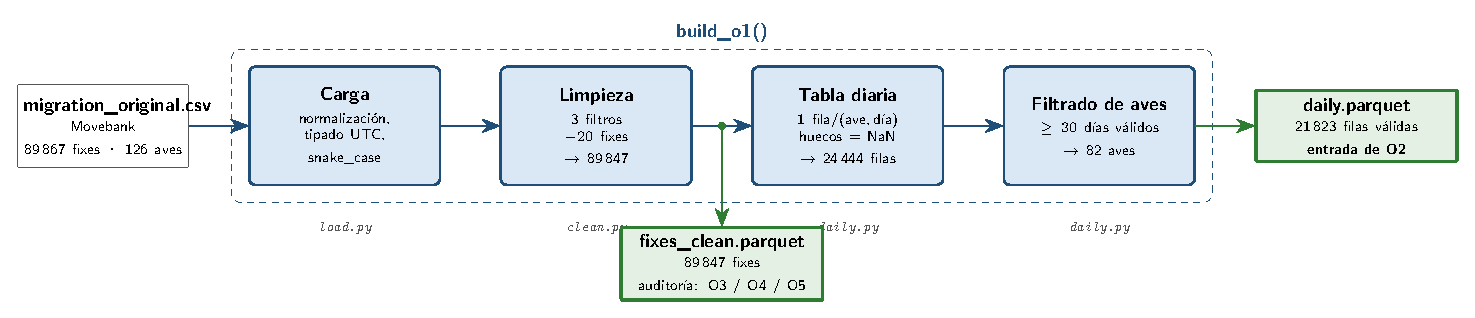
\includegraphics[width=\linewidth]{o1_pipeline.pdf}
  \caption[Canalización de preparación de datos]{Canalización de
  preparación de datos. A partir del fichero crudo de Movebank, las cuatro
  etapas (carga, limpieza, tabla diaria y filtrado de individuos) producen dos
  salidas: \texttt{daily.parquet}, la tabla diaria que alimenta el modelo de
  Markov, y \texttt{fixes\_clean.parquet}, los \textit{fixes} limpios que se
  reservan como material de auditoría para los objetivos posteriores.}
  \label{fig:o1-pipeline}
\end{figure}

La tabla diaria es la única entrada del modelo de Markov del capítulo siguiente,
por lo que las decisiones sobre granularidad y representación de huecos
condicionan directamente su diseño. La canalización conserva además los
\textit{fixes} limpios a su resolución original, antes del submuestreo, como
material de auditoría: de ahí se extraerán variables cinemáticas para la detección
de comportamiento y los modelos supervisados.

\section{El conjunto de datos de partida}
\label{sec:o1-dataset}

\subsection{Origen, especie y experimento}
\label{sec:o1-origen}

Los datos proceden del repositorio Movebank, del estudio \textit{Navigation
experiments in lesser black-backed gulls} \cite{movebank_gulls}, asociado a los
experimentos de navegación de Wikelski et al. \cite{wikelski2015}. Recogen el
seguimiento GPS de gaviotas sombrías (\textit{Larus fuscus}) entre 2009 y 2015.
Todos los individuos pertenecen a la misma especie: no hay variabilidad
interespecífica, de modo que las diferencias que se observen son atribuibles a la
variación individual, estacional o geográfica, no a la especie. Esta homogeneidad
simplifica la interpretación de los modelos y permite tratar a los individuos como
variantes de un mismo patrón migratorio.

\subsection{Formato y selección de variables}
\label{sec:o1-variables}

El conjunto sigue el formato estándar de Movebank, en el que cada fila es un
\textit{fix} y las columnas se agrupan en cuatro familias:

\begin{itemize}
  \item \emph{Identificación y contexto:} el identificador único del evento
  (\texttt{event-id}), el del individuo (\texttt{individual-local-identifier}) y
  el tipo de sensor (\texttt{sensor-type}), que en este conjunto es siempre GPS.
  \item \emph{Espacio-temporales:} la marca temporal (\texttt{timestamp}) y las
  coordenadas geográficas en grados decimales (\texttt{location-long} y
  \texttt{location-lat}).
  \item \emph{Calidad y control:} los indicadores \texttt{visible} y
  \texttt{manually-marked-outlier}, que señalan los registros que el propio
  repositorio marca como no visibles o como atípicos por inspección.
  \item \emph{Ambientales:} covariables de modelos climáticos externos, como la
  cobertura de vegetación baja y alta de ECMWF o la vegetación superficial de
  NCEP\@.
\end{itemize}

De ahí se selecciona el subconjunto de variables imprescindible para el modelado y
se renombra a una nomenclatura uniforme en \textit{snake\_case} (tabla
\ref{tab:o1-variables}). Se descartan los metadatos administrativos (nombre del
estudio, identificador físico de la etiqueta y nombre taxonómico, redundante al
haber una sola especie) y, en este objetivo, también las covariables ambientales:
no intervienen en la tabla diaria y, en el caso de la vegetación de NCEP, están
ausentes en todo el conjunto. El identificador de individuo se conserva como
cadena de texto (por ejemplo, \texttt{91732A}), ya que es una etiqueta y no un
valor numérico.

\begin{table}[H]
  \centering
  \caption[Selección y renombrado de variables]{Subconjunto de variables del
  formato Movebank conservadas en este capítulo, con su nombre en el proyecto y su uso. El
  resto de columnas (metadatos administrativos y covariables ambientales) se
  descarta.}
  \label{tab:o1-variables}
  \begin{tabular}{lll}
    \toprule
    \textbf{Columna Movebank} & \textbf{Nombre en el proyecto} & \textbf{Uso} \\
    \midrule
    \texttt{event-id} & \texttt{event\_id} & Identificador del \textit{fix} \\
    \texttt{timestamp} & \texttt{timestamp} & Eje temporal (UTC) \\
    \texttt{location-long} & \texttt{lon} & Longitud \\
    \texttt{location-lat} & \texttt{lat} & Latitud \\
    \texttt{individual-local-identifier} & \texttt{bird\_id} & Identificador del individuo \\
    \texttt{visible} & \texttt{visible} & Control de calidad \\
    \texttt{manually-marked-outlier} & \texttt{manually\_marked\_outlier} & Control de calidad \\
    \texttt{sensor-type} & \texttt{sensor\_type} & Tipo de sensor (siempre GPS) \\
    \bottomrule
  \end{tabular}
\end{table}

\subsection{Caracterización inicial}
\label{sec:o1-caracterizacion}

Tras la carga, el conjunto comprende 89\,867 \textit{fixes} de 126 individuos a
lo largo de algo más de seis años (tabla \ref{tab:o1-overview}). La cobertura por
individuo es marcadamente asimétrica: la mediana es de 262 \textit{fixes}, pero el
percentil 10 baja a 26 y el percentil 90 asciende a 1\,533. Coexisten, por tanto,
aves con un seguimiento denso y prolongado y aves con un rastro esporádico. Esta
disparidad anticipa la necesidad de un criterio de admisión por individuo, que se
introduce más adelante en este capítulo.

\begin{table}[H]
  \centering
  \caption[Caracterización del conjunto crudo]{Métricas agregadas del conjunto
  crudo de Movebank tras la carga y normalización.}
  \label{tab:o1-overview}
  \begin{tabular}{lr}
    \toprule
    \textbf{Métrica} & \textbf{Valor} \\
    \midrule
    \textit{Fixes} GPS totales & 89\,867 \\
    Individuos (\textit{Larus fuscus}) & 126 \\
    Mediana de \textit{fixes} por individuo & 262 \\
    Percentil 10 / 90 de \textit{fixes} por individuo & 26 / 1\,533 \\
    Primer registro (UTC) & 2009-05-25 \\
    Último registro (UTC) & 2015-08-27 \\
    \bottomrule
  \end{tabular}
\end{table}

\section{Limpieza de los \textit{fixes} GPS}
\label{sec:o1-limpieza}

La limpieza aplica primero varias comprobaciones de integridad estándar: descarta
los \textit{fixes} que el repositorio marca como no válidos (indicadores
\texttt{visible} y \texttt{manually-marked-outlier}), las coordenadas fuera del
rango geográfico físico y los registros duplicados en
\texttt{(bird\_id, timestamp)}. Ninguna de ellas elimina registros en este
conjunto, lo que indica que los datos se distribuyen ya parcialmente depurados. El
único filtro con efecto es el de velocidad, que reduce los 89\,867 \textit{fixes}
iniciales a 89\,847 (el 99,98\,\% del total).

Este filtro compara la velocidad implícita entre \textit{fixes} consecutivos del
mismo individuo con un máximo admisible. La
distancia entre dos posiciones se calcula con la fórmula de Haversine, que da la
distancia sobre la superficie de la esfera:

\begin{equation}
  d = 2R \arcsin\sqrt{\sin^2\!\frac{\Delta\phi}{2}
      + \cos\phi_1 \cos\phi_2 \sin^2\!\frac{\Delta\lambda}{2}},
  \label{eq:haversine}
\end{equation}

donde $\phi$ es la latitud, $\lambda$ la longitud (en radianes), $\Delta\phi$ y
$\Delta\lambda$ sus diferencias entre los dos \textit{fixes} y
$R = 6371{,}0088$ km el radio medio terrestre. La velocidad implícita es
$v = d/\Delta t$, con $\Delta t$ el intervalo entre ambos.

El umbral se fija en 120 km/h, valor que justifica la distribución de velocidades
(figura \ref{fig:o1-speed}). La mediana es de 0,66 km/h y el percentil 99,5 es de
50,6 km/h, en línea con la velocidad de crucero de \textit{Larus fuscus} (unos
50 km/h); solo el extremo de la cola (percentil 99,9 en 134 km/h) alcanza valores
incompatibles con el vuelo del ave. El umbral queda por encima del régimen de
crucero y de su margen con viento favorable, de modo que aísla los artefactos del
GPS sin penalizar desplazamientos legítimos.

Un único \textit{fix} erróneo contamina dos velocidades: la del segmento que llega
a él y la del que parte de él. Para no penalizar a sus vecinos legítimos, el filtro
es iterativo. En cada iteración elimina solo el \textit{fix} de mayor velocidad (el
responsable más probable) y recalcula las velocidades de los vecinos en la
siguiente, hasta que ninguna supera el umbral o hasta un tope de 20 iteraciones.
Sobre este conjunto el filtro alcanza ese tope sin converger por completo, pero su
efecto es marginal: descarta 20 \textit{fixes} (el 0,022\,\% del total).

\begin{figure}[H]
  \centering
  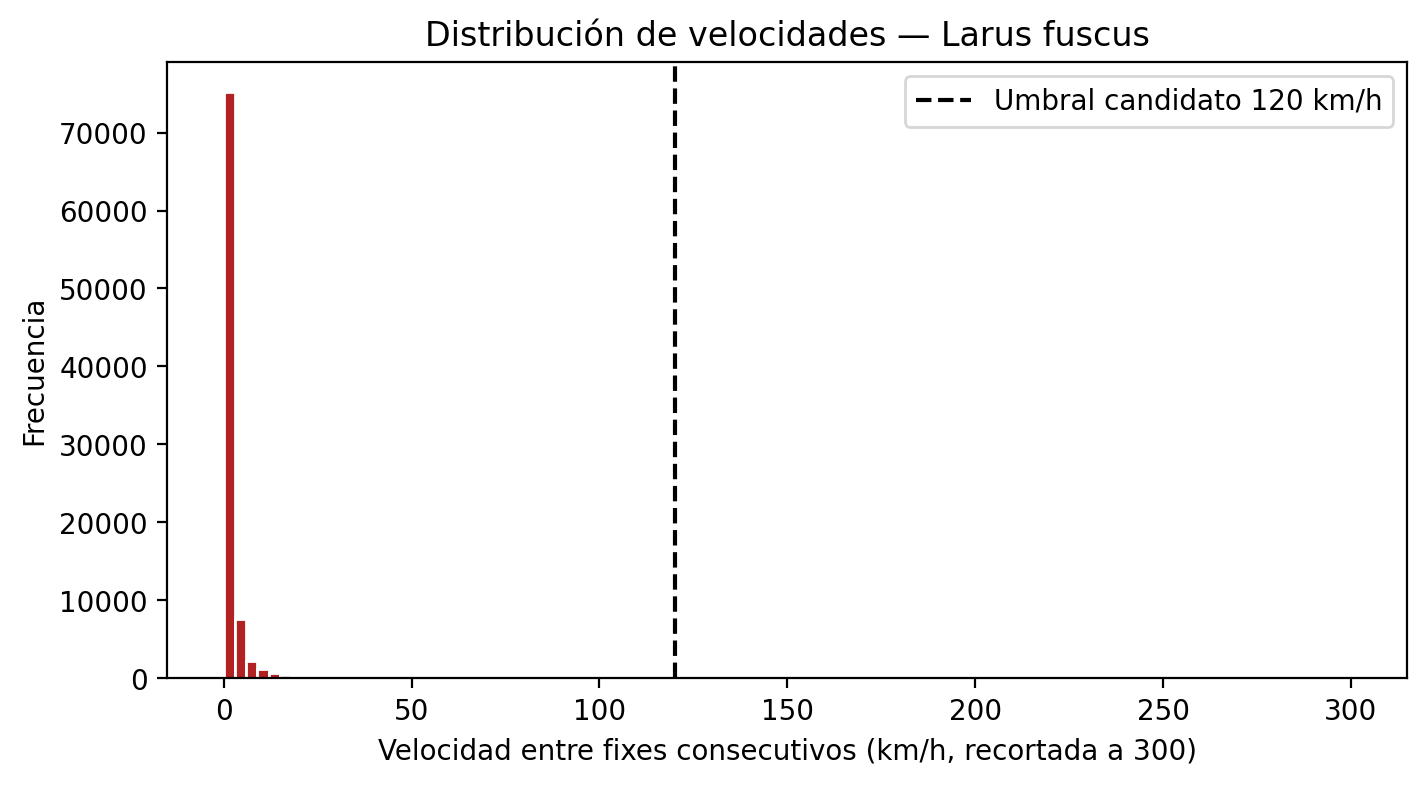
\includegraphics[width=0.85\linewidth]{o1_fig03_speed-distribution.png}
  \caption[Distribución de velocidades entre \textit{fixes}]{Distribución de las
  velocidades entre \textit{fixes} consecutivos del mismo individuo. Casi todos los
  valores se concentran muy por debajo de la velocidad de crucero de la especie; el
  umbral de 120 km/h (línea discontinua) deja un margen amplio sobre ese régimen y
  aísla los artefactos del GPS sin penalizar desplazamientos legítimos.}
  \label{fig:o1-speed}
\end{figure}

\section{Construcción de la tabla diaria}
\label{sec:o1-resample}

Con los \textit{fixes} ya limpios, el último paso reduce la trayectoria de cada
individuo a una posición por día natural (UTC): para cada día se toma el
\textit{fix} más cercano a una hora de referencia fija, y los días sin un
\textit{fix} suficientemente próximo quedan como huecos.

\subsection{Hora de referencia}
\label{sec:o1-hora}

La hora de referencia debe coincidir con uno de los picos de muestreo: fuera de
ellos hay muy pocos \textit{fixes}, y cualquier otra hora dejaría la mayoría de los
días sin una observación cercana. Esto reduce la elección a las cuatro ventanas en
que se concentra el muestreo (05:00, 08:00, 14:00 y 20:00 UTC), de volumen casi
idéntico (entre 15\,466 y
15\,656 \textit{fixes}; figura \ref{fig:o1-hourly}), por lo que el volumen no decide
entre ellas. La elección concreta de las 08:00 responde a un criterio biológico:
coinciden con el inicio del ciclo diario de actividad de \textit{Larus fuscus} en
buena parte de su rango migratorio, por lo que la posición a esa hora corresponde al
lugar de descanso nocturno (\textit{roost}) o al punto inmediatamente posterior al
despegue, un estado espacialmente estable. El anclaje
favorece además al modelo de Markov: observar el origen y el destino de cada
transición en el mismo punto del ciclo diario hace las transiciones comparables
entre días.

\begin{figure}[H]
  \centering
  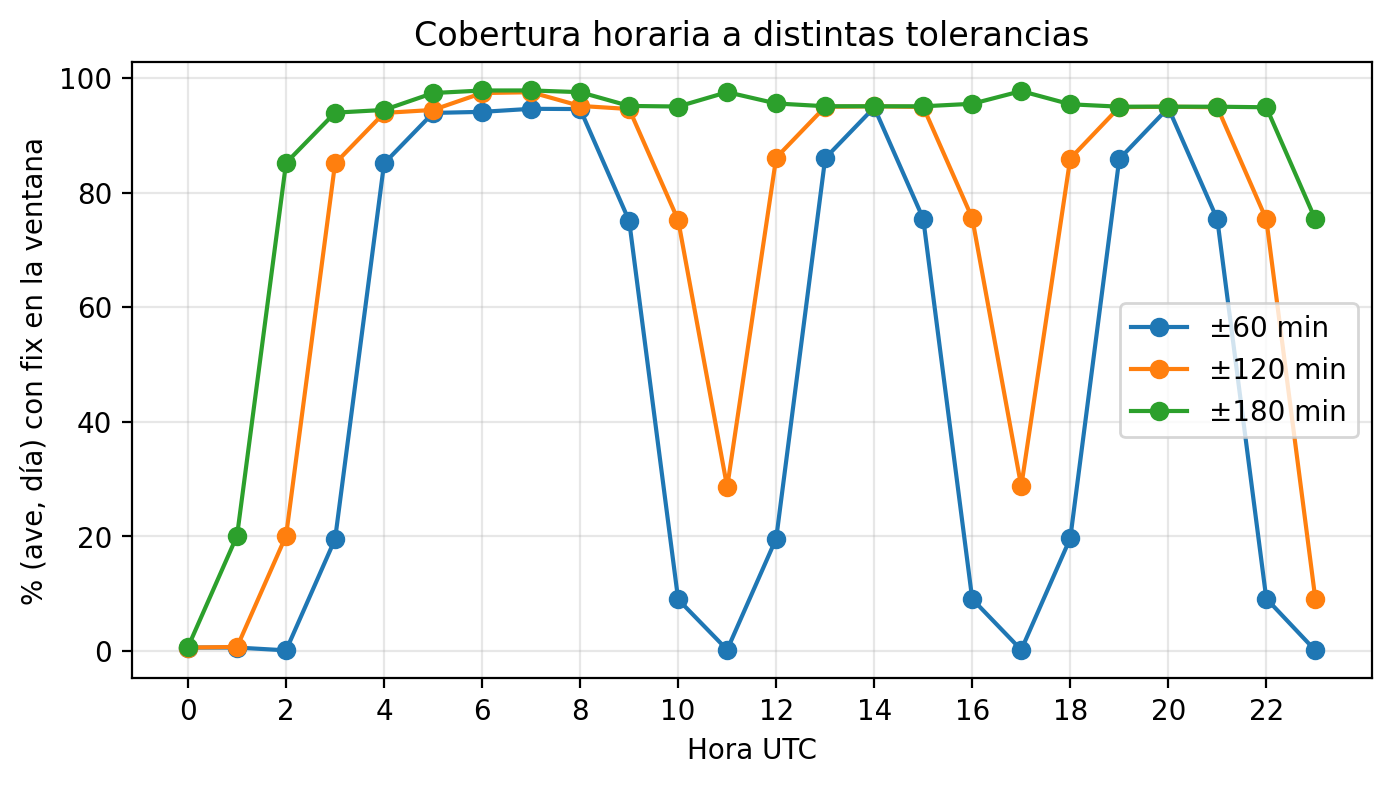
\includegraphics[width=0.85\linewidth]{o1_fig04_hourly-coverage.png}
  \caption[Distribución horaria de los \textit{fixes}]{Número de \textit{fixes} por
  hora UTC tras la limpieza. El muestreo se concentra en cuatro ventanas (05:00,
  08:00, 14:00 y 20:00 UTC) de volumen casi idéntico; la ventana sombreada marca la
  elegida (08:00 $\pm$ 60 min).}
  \label{fig:o1-hourly}
\end{figure}

\subsection{Selección por cercanía y huecos explícitos}
\label{sec:o1-seleccion}

De cada día se conserva el \textit{fix} más cercano a la hora de referencia, medido
por su distancia temporal en minutos (\texttt{delta\_minutes}); no se interpola una
posición intermedia, en coherencia con el principio de no introducir datos no
observados. Un \textit{fix} se acepta como representante del día solo si cae dentro
de una ventana de tolerancia de $\pm 60$ min alrededor de las 08:00, holgada a
propósito para no fragmentar la serie con huecos innecesarios: con $\pm 60$ min se
conserva el 94,6\,\% de los días, frente al 66\,\% que dejaría una ventana estrecha
de $\pm 30$ min. No se amplía más porque entonces mezclaría posiciones de puntos
distintos del ciclo diario. Para
los días sin \textit{fix} válido, el procedimiento reconstruye el calendario completo de cada
individuo entre su primera y su última observación e inserta una fila por cada día
ausente, marcada como no válida y con coordenadas nulas. De este modo los huecos son
explícitos: una fila registrada, no una discontinuidad implícita.

La figura \ref{fig:o1-timeline} muestra el resultado para un individuo (91916A):
rachas largas de días válidos intercaladas con huecos puntuales o de varios días.
Esta heterogeneidad es habitual en el conjunto y es la razón de representar los
huecos en lugar de eliminarlos. Un modelo de transición día a día que encontrara dos
observaciones separadas por un hueco no anotado las trataría como días consecutivos e
introduciría un salto espacial inexistente.

\begin{figure}[H]
  \centering
  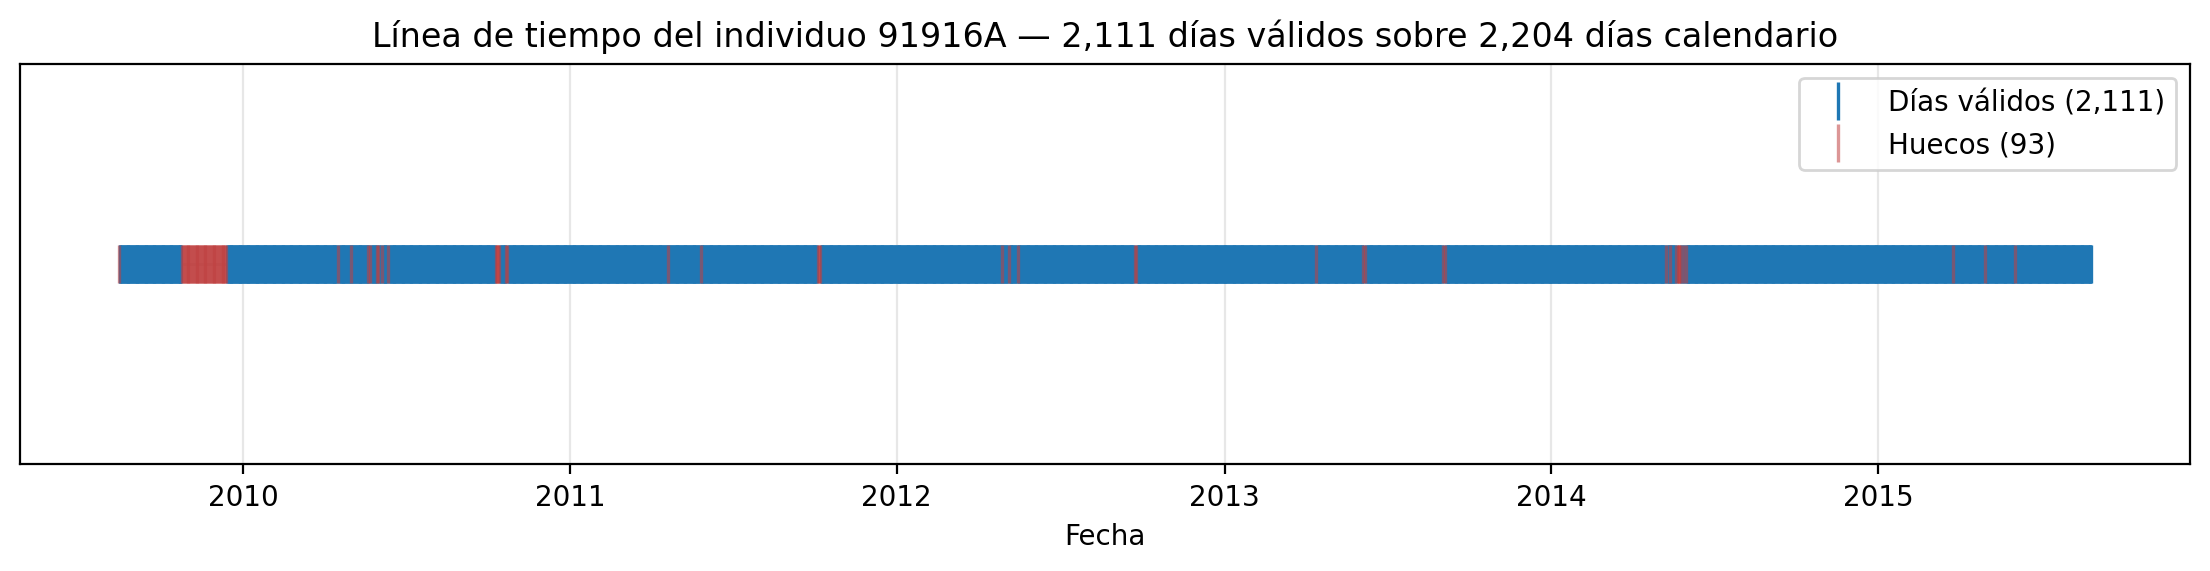
\includegraphics[width=0.85\linewidth]{o1_fig11_timeline-91916a.png}
  \caption[Línea de tiempo de un individuo]{Línea de tiempo del individuo 91916A
  tras el resample. En azul, los días con \textit{fix} válido (08:00 UTC
  $\pm$ 60 min); en rojo, los huecos. Alterna rachas largas de continuidad con
  huecos puntuales o de varios días, un patrón habitual en el conjunto.}
  \label{fig:o1-timeline}
\end{figure}

\section{Filtrado de individuos y dataset final}
\label{sec:o1-final}

\subsection{Umbral de días válidos}
\label{sec:o1-umbral}

El resample genera días válidos y huecos para cada individuo, pero no todos tienen
suficiente historia para estimar transiciones. El último filtro descarta los
individuos con menos de 30 días válidos. La figura \ref{fig:o1-validdays} muestra la
distribución de días válidos por individuo y el número de aves que supera distintos
umbrales. Con 30 días se conservan 82 de los 126 individuos (el 65\,\%). Un umbral
más laxo retendría más aves, pero a costa de admitir rastros demasiado escasos para
estimar transiciones; uno más estricto sacrificaría muestra útil. El corte en 30
días equilibra ambos extremos.

\begin{figure}[H]
  \centering
  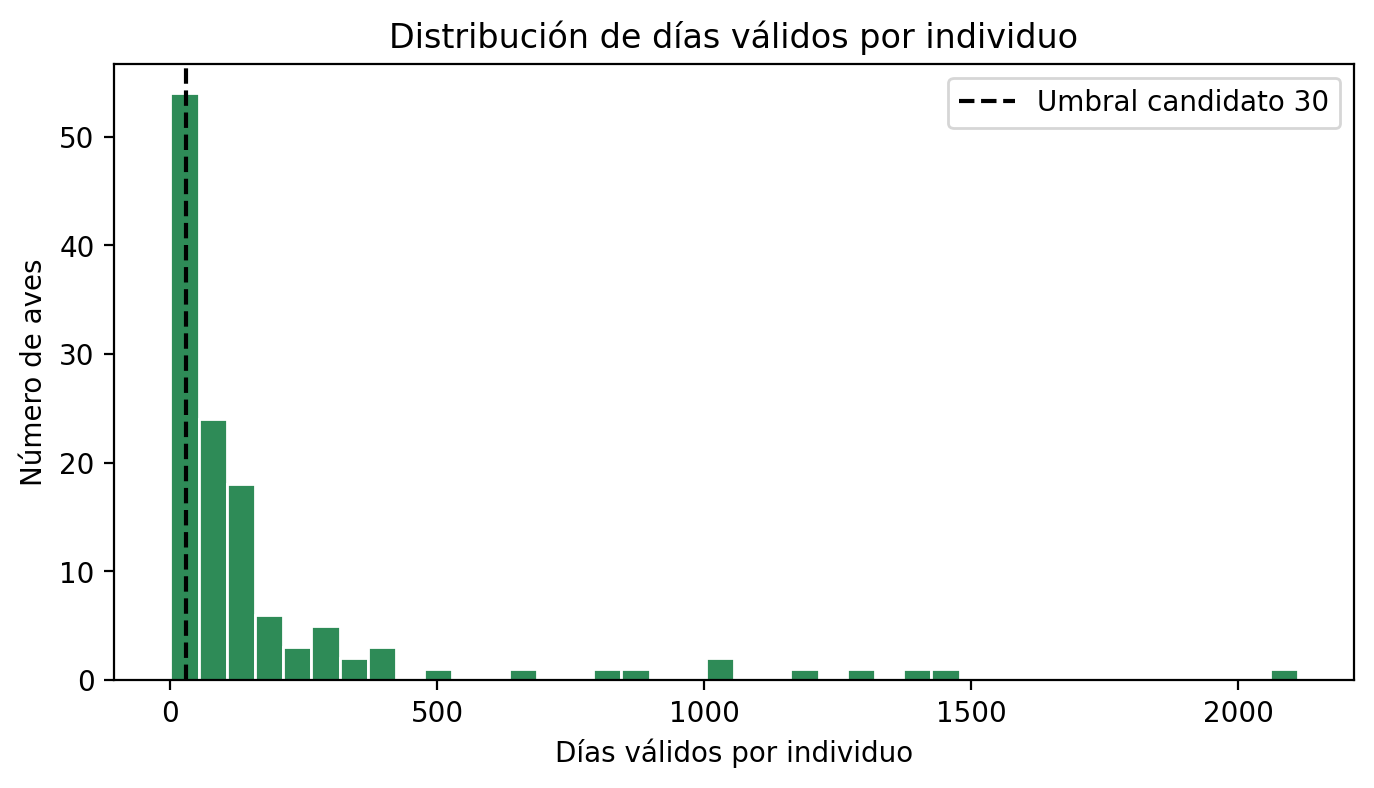
\includegraphics[width=0.85\linewidth]{o1_fig06_valid-days-per-bird.png}
  \caption[Días válidos por individuo]{Distribución del número de días válidos por
  individuo y número de aves conservadas según el umbral. El corte en 30 días
  descarta los individuos con seguimiento insuficiente para el modelo de Markov sin
  penalizar a la mayoría del conjunto.}
  \label{fig:o1-validdays}
\end{figure}

\subsection{El conjunto de datos final}
\label{sec:o1-dataset-final}

La tabla \ref{tab:o1-funnel} resume la reducción de los datos a lo largo de la
pipeline.

\begin{table}[H]
  \centering
  \caption[Reducción de los datos a lo largo de la pipeline]{Reducción del volumen
  de datos en cada etapa, desde los \textit{fixes} en bruto hasta la tabla diaria
  final.}
  \label{tab:o1-funnel}
  \begin{tabular}{lr}
    \toprule
    \textbf{Etapa} & \textbf{Recuento} \\
    \midrule
    \textit{Fixes} GPS brutos (126 individuos) & 89\,867 \\
    \textit{Fixes} tras la limpieza & 89\,847 \\
    Individuos conservados ($\geq 30$ días válidos) & 82 \\
    Filas de la tabla diaria final & 24\,444 \\
    Filas válidas (con posición real) & 21\,823 \\
    \bottomrule
  \end{tabular}
\end{table}

La pipeline produce dos ficheros: \texttt{daily.parquet}, la tabla diaria que
alimenta el modelo de Markov, y \texttt{fixes\_clean.parquet}, los \textit{fixes}
limpios a su resolución original, reservados como material de auditoría para los
objetivos posteriores. Ambos se regeneran con una sola llamada a
\texttt{build\_o1()}; sus funciones de carga, limpieza y resample son puras y solo
el orquestador escribe a disco.

\section{Caracterización del dataset resultante}
\label{sec:o1-resultante}

La tabla diaria es la entrada del modelo de Markov del capítulo siguiente. Tres
propiedades del conjunto resultante condicionan cómo puede explotarse: su cobertura
espacial, la fragmentación de las series y el sesgo estacional del seguimiento.

\subsection{Dominio espacial}
\label{sec:o1-espacial}

Los \textit{fixes} conservados cubren el corredor migratorio completo de la especie,
desde las zonas de cría en el norte de Europa hasta las áreas de invernada en el
este de África (figura \ref{fig:o1-spatial}). Esta extensión fija el dominio que
la cadena de Markov deberá discretizar: la rejilla de celdas ha de abarcar desde las
latitudes nórdicas hasta el este de África.

\begin{figure}[H]
  \centering
  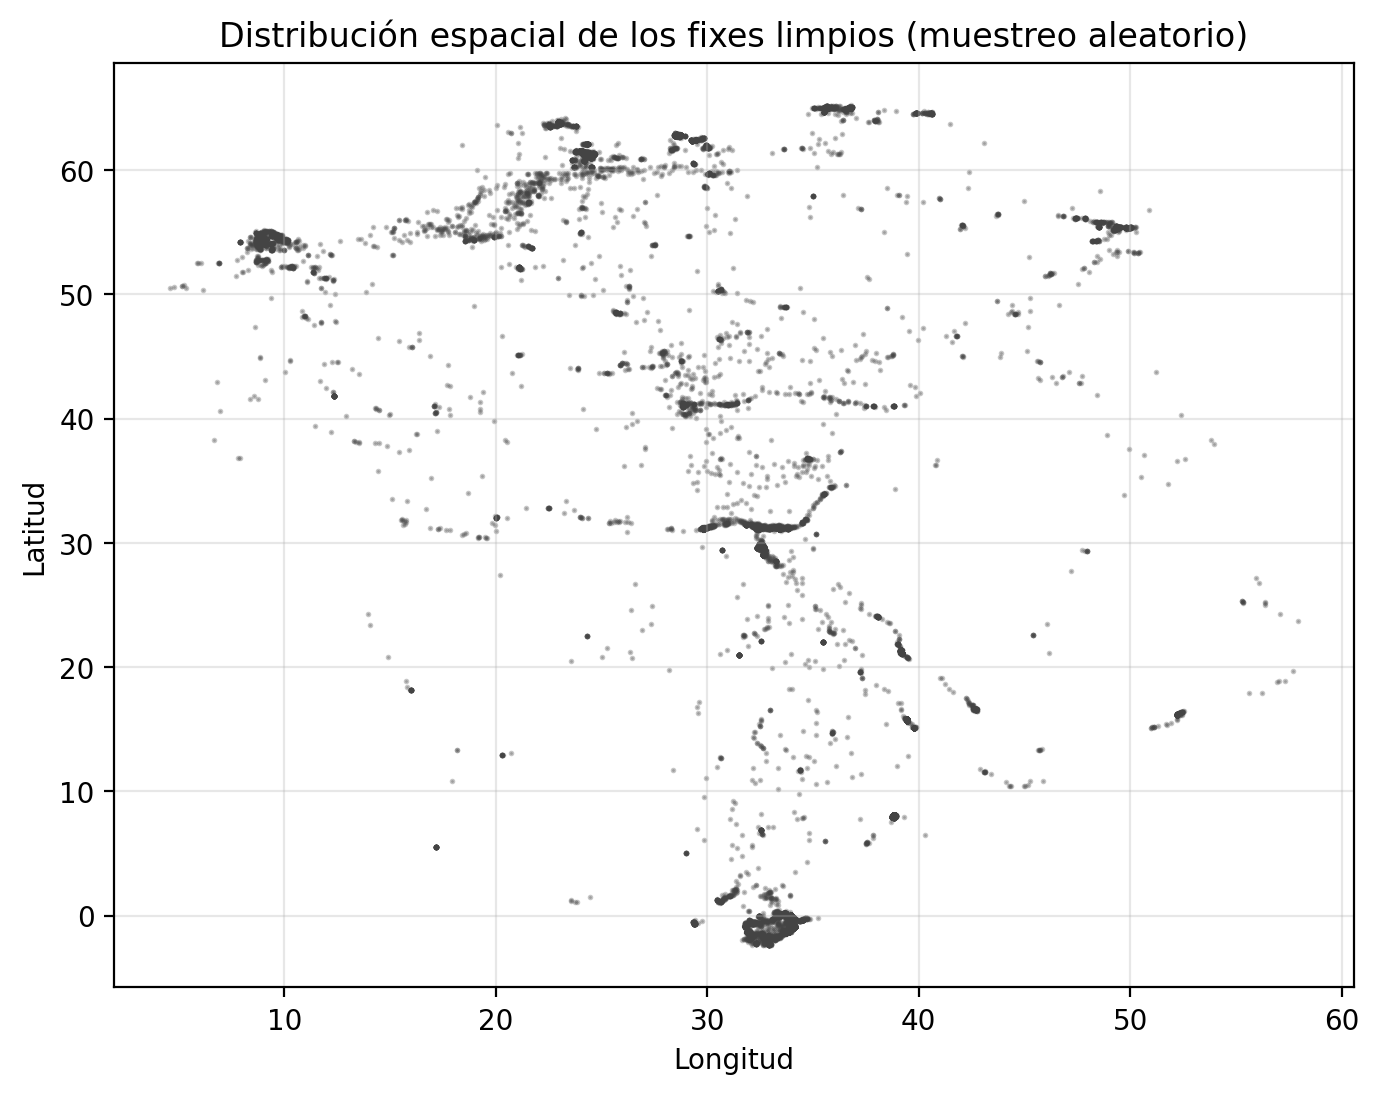
\includegraphics[width=0.85\linewidth]{o1_fig08_spatial-overview.png}
  \caption[Distribución geográfica de los \textit{fixes}]{Distribución geográfica de
  una muestra de los \textit{fixes} conservados. El conjunto cubre el corredor
  migratorio de \textit{Larus fuscus} entre el norte de Europa y el este de
  África.}
  \label{fig:o1-spatial}
\end{figure}

\subsection{Fragmentación de las series}
\label{sec:o1-fragmentacion}

Las rachas de días válidos consecutivos son en su mayoría cortas: la mediana es de
8 días (figura \ref{fig:o1-streak}). Para el modelo de Markov esto supone abundancia
de transiciones de un solo paso, pero escasez de tramos largos continuos en la mayor
parte de la muestra. Queda abierta para ese modelo una decisión: entrenar sobre
todas las rachas o exigir una longitud mínima.

\begin{figure}[H]
  \centering
  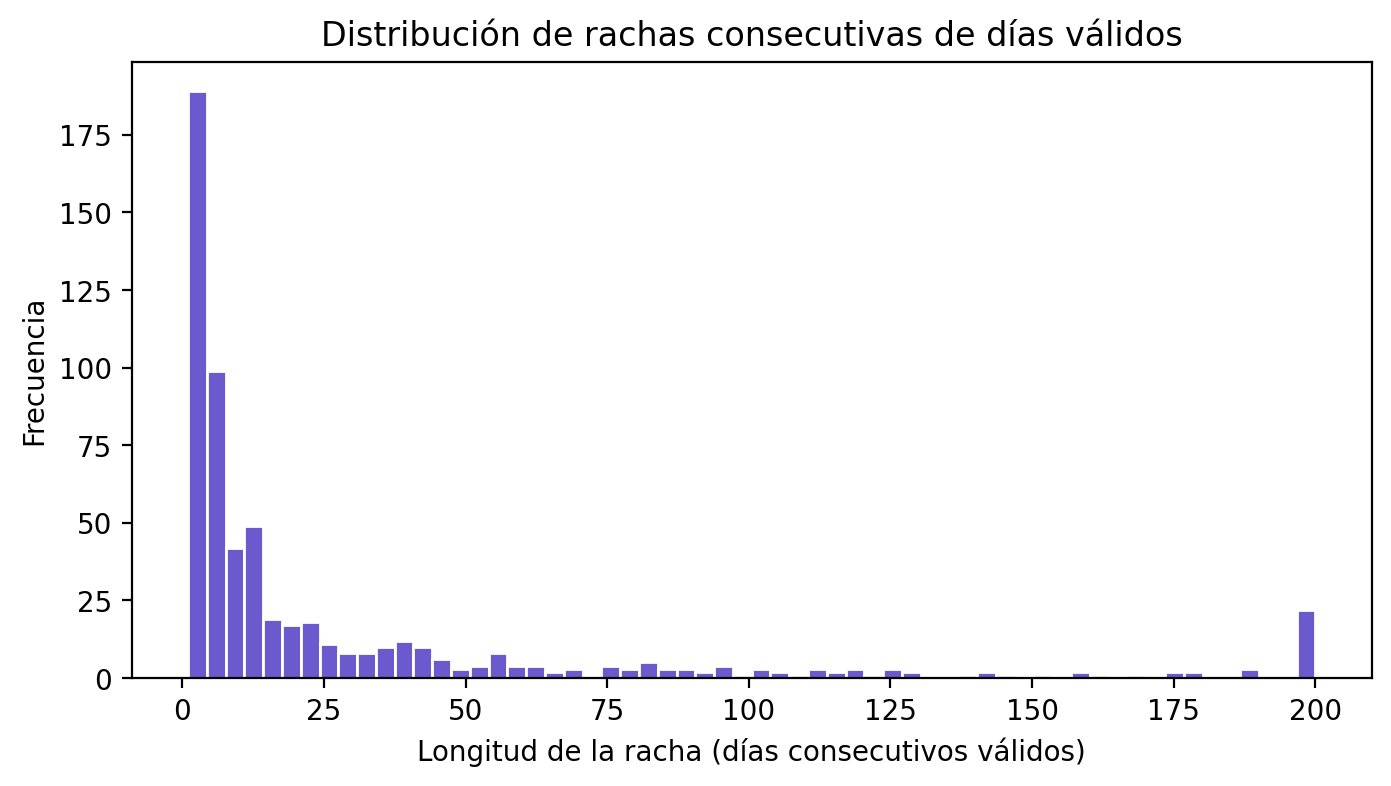
\includegraphics[width=0.85\linewidth]{o1_fig09_streak-length-distribution.png}
  \caption[Longitud de las rachas de días válidos]{Distribución de la longitud de
  las rachas de días válidos consecutivos en la tabla diaria (eje recortado a 200
  días). La mayoría son cortas (mediana de 8 días), con una cola larga de aves
  seguidas de forma casi continua durante meses.}
  \label{fig:o1-streak}
\end{figure}

\subsection{Sesgo estacional del seguimiento}
\label{sec:o1-estacional}

El seguimiento no se reparte por igual a lo largo del año (figura
\ref{fig:o1-seasonal}). El otoño reúne casi el doble de observaciones válidas que la
primavera, con un máximo en septiembre y un mínimo en mayo; en términos de
fenología, la migración de otoño queda mucho mejor muestreada que la de primavera.
En consecuencia, las transiciones que el modelo estime para las estaciones bien
representadas se apoyarán en más datos que las de las estaciones escasas, algo a
tener en cuenta al interpretar su precisión por régimen.

\begin{figure}[H]
  \centering
  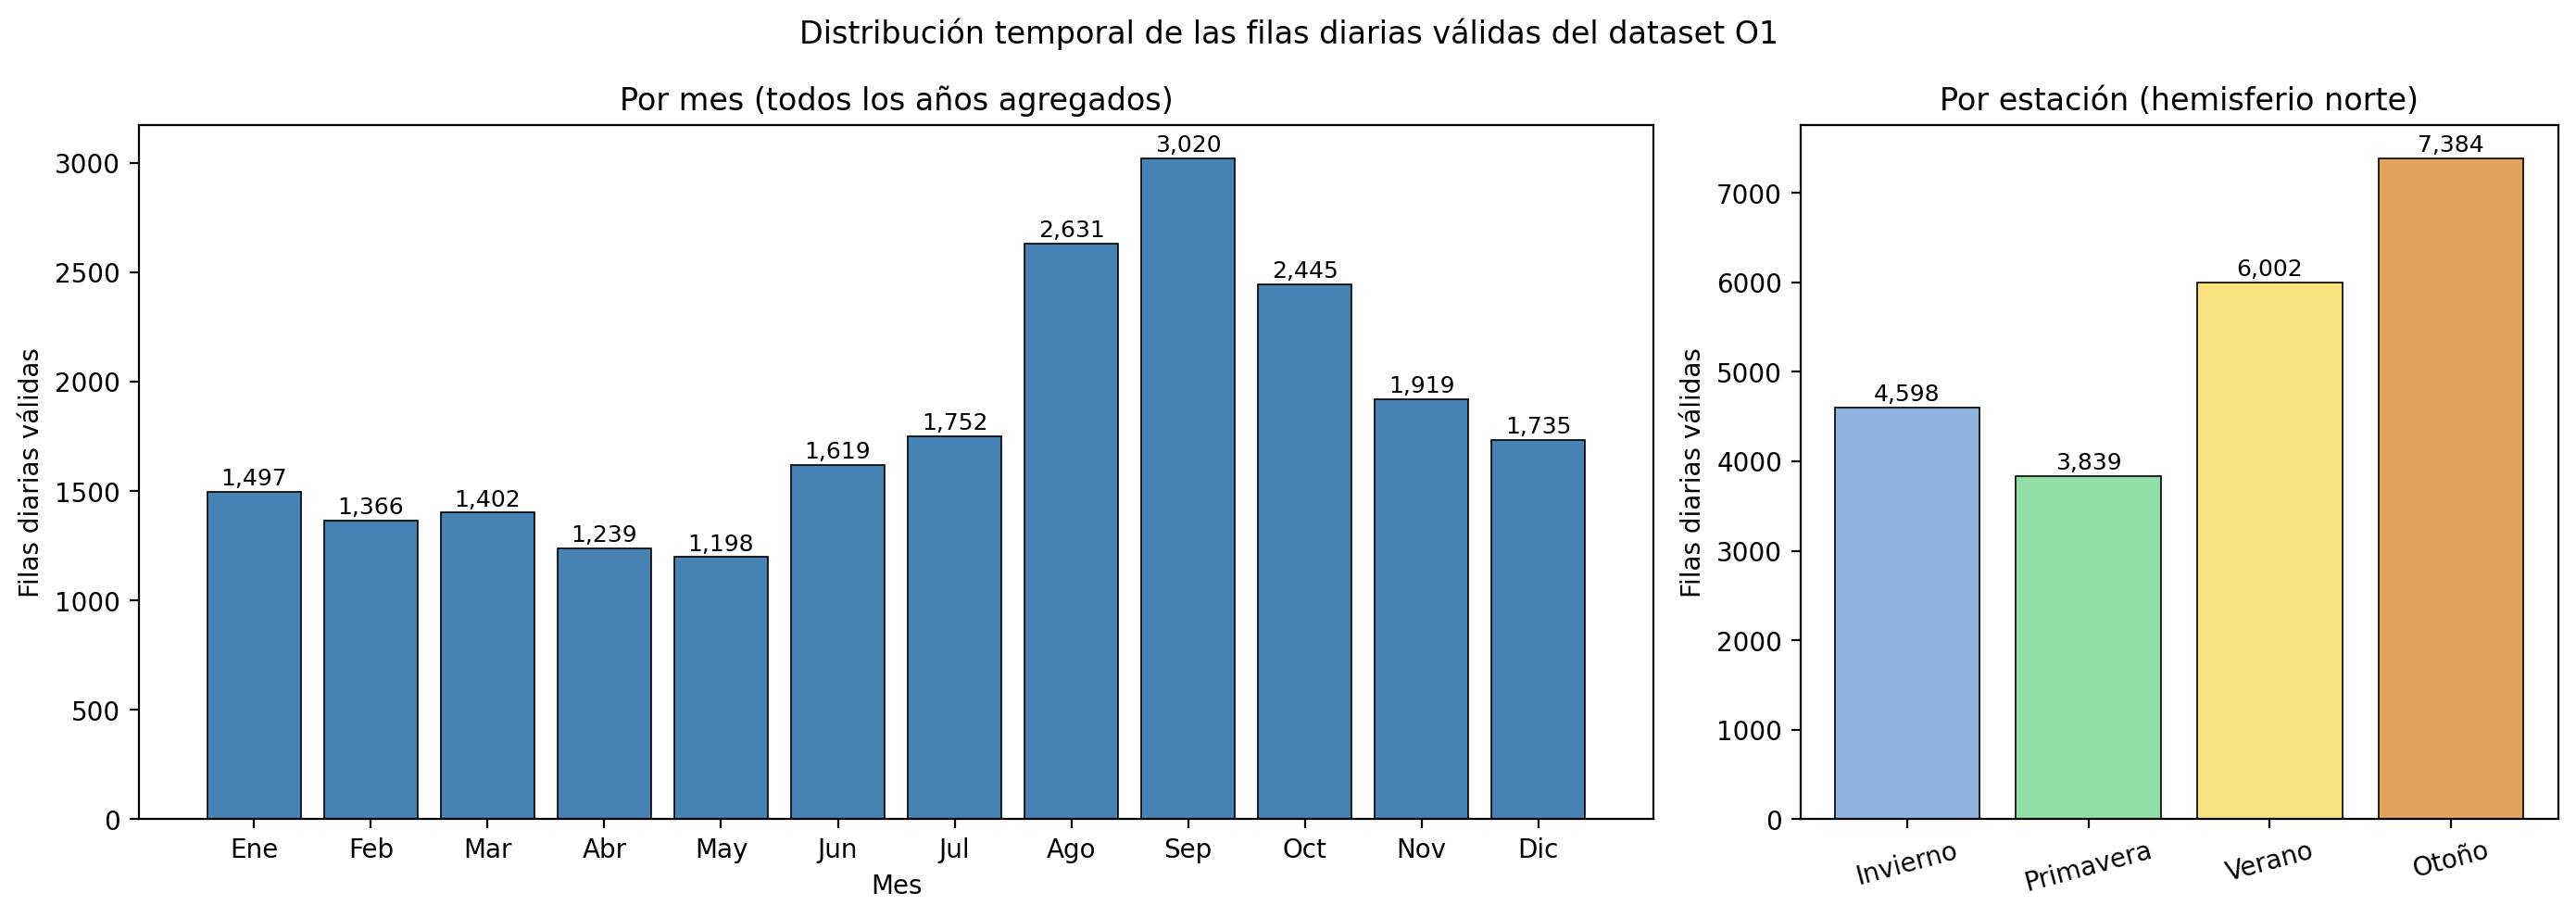
\includegraphics[width=0.85\linewidth]{o1_fig10_monthly-seasonal-coverage.png}
  \caption[Cobertura mensual y estacional]{Filas diarias válidas por mes y por
  estación (hemisferio norte). El seguimiento se concentra en el otoño y es escaso
  en primavera, un sesgo que condiciona la interpretación de las transiciones por
  estación.}
  \label{fig:o1-seasonal}
\end{figure}

\chapter{Predicción con cadenas de Markov visibles}
\label{ch:o2}

Este capítulo construye el primer modelo predictivo del trabajo: una cadena de
Markov de primer orden que, a partir de la celda en la que un individuo se
encuentra hoy, estima en cuál estará mañana. Se llama \emph{visible} porque su
estado (la celda ocupada) es una variable observada directamente, a diferencia de
los estados ocultos que introducirá el capítulo siguiente. Más allá de su interés
propio, el modelo cumple un papel transversal: es la referencia interpretable y
cuantificada que los modelos posteriores (capítulos \ref{ch:o3} y \ref{ch:o4})
deberán superar.

\section{Introducción y objetivo}
\label{sec:o2-intro}

La entrada de este objetivo es la tabla diaria producida en el capítulo
\ref{ch:o1}: una posición por individuo y día natural (UTC), con los huecos
representados de forma explícita y la posición anclada a las 08:00, próxima al
lugar de descanso nocturno (\textit{roost}). Sobre esa secuencia regular se
plantea la pregunta de predicción más simple posible: dado dónde está hoy el ave,
¿dónde estará mañana? El modelo que la responde con menos supuestos, respetando la
estructura temporal de la serie, es una cadena de Markov de primer orden sobre el
espacio discretizado.

La discretización convierte cada posición diaria en un estado: el dominio
geográfico se divide en una rejilla de celdas y la posición del día $t$ se
identifica con la celda que la contiene, $X_t$, dentro de un espacio finito de $N$
celdas. La hipótesis de Markov de primer orden establece que la celda del día
siguiente depende solo de la celda actual, no de toda la trayectoria previa:

\begin{equation}
  P(X_{t+1} = j \mid X_t = i,\, X_{t-1}, \dots, X_0)
  = P(X_{t+1} = j \mid X_t = i) = p_{ij},
  \label{eq:o2-markov}
\end{equation}

donde $p_{ij}$ es la probabilidad de transitar de la celda $i$ a la $j$. El
conjunto de estas probabilidades forma la matriz de transición $P$, con
$\sum_j p_{ij} = 1$ para toda celda de origen. Para captar la estacionalidad del
ciclo migratorio, el modelo no usa una única matriz sino una por mes natural,
$P^{(m)}$ con $m = 1, \dots, 12$. La teoría general de las cadenas de Markov
finitas se trata en el capítulo \ref{ch:preliminares}; aquí se emplea en su forma
aplicada al problema.

La cuestión concreta del capítulo es si una cadena de Markov de primer orden,
global (una sola familia de matrices compartida por todos los individuos) y con
estacionalidad mensual, mejora a la predicción trivial de \emph{persistencia}
(suponer que mañana el ave seguirá en la misma celda que hoy). Esta baseline no es
un rival ingenuo: como se verá, la marcada tendencia de la especie a permanecer en
el mismo lugar la hace sorprendentemente difícil de batir, y esa dificultad es,
por sí misma, un resultado. El modelo de Markov aporta además el criterio de
comparación cuantificado que reutilizan los objetivos siguientes: sus predicciones
se almacenan para el análisis comparativo del error del capítulo \ref{ch:o5}.

\section{Discretización del espacio}
\label{sec:o2-discretizacion}

El primer paso convierte la posición continua en un estado discreto. El dominio
geográfico se cubre con una rejilla de celdas cuadradas de lado \texttt{cell\_deg}
grados, y cada posición $(\texttt{lon}, \texttt{lat})$ se asigna a la celda que la
contiene, identificada por su índice de latitud
$\lfloor \texttt{lat} / \texttt{cell\_deg} \rfloor$ y su índice de longitud
$\lfloor \texttt{lon} / \texttt{cell\_deg} \rfloor$ (por ejemplo, \texttt{122\_49}). Solo se conservan como estados las celdas con al
menos una observación válida, que forman el espacio de celdas activas. Con ello la
posición diaria de un individuo queda reducida a la secuencia de celdas $X_t$ sobre
la que opera la cadena.

El tamaño de celda no es un parámetro inocuo: fija a la vez la resolución espacial
del modelo y la proporción de \emph{self-loops} (transiciones que permanecen en la
misma celda de un día al siguiente), que es justamente la magnitud de la que
depende la fortaleza de la baseline de persistencia. Una celda demasiado grande
hace que casi todos los días parezcan estacionarios y una demasiado pequeña deja
sin datos a la mayoría de las transiciones, así que la elección se decide
comparando cuatro candidatos (0,25\textdegree, 0,5\textdegree, 1\textdegree\ y
2\textdegree; figura \ref{fig:o2-grid}).

El compromiso es claro en los extremos. Con celdas de 2\textdegree\ (del orden de
222 km) el 86,1\,\% de las transiciones son self-loops: el movimiento migratorio
que el modelo debería capturar se diluye dentro de la celda y la persistencia se
infla por construcción. Con celdas de 0,25\textdegree\ (unos 28 km) la resolución
es fina pero la estimación se vuelve inviable, porque en un mes típico cada celda
registra menos de una transición (la mediana de transiciones por celda y mes es
0,86; panel B de la figura), de modo que la mayoría de las celdas se queda sin datos
con los que estimar sus probabilidades. El tamaño intermedio de \textbf{0,5\textdegree}
(del orden de 56 km) es comparable a la escala del grueso de los desplazamientos
diarios (panel A de la figura): un día de movimiento real cruza varias celdas
mientras que un día de descanso permanece en la misma. A esa resolución el espacio
tiene 1\,217 celdas activas y el 73,0\,\% de las transiciones son self-loops, una
residencialidad alta pero no exagerada y coherente con la fenología de la especie.
Se adopta, por tanto, \texttt{cell\_deg} = 0,5\textdegree.

\begin{figure}[H]
  \centering
  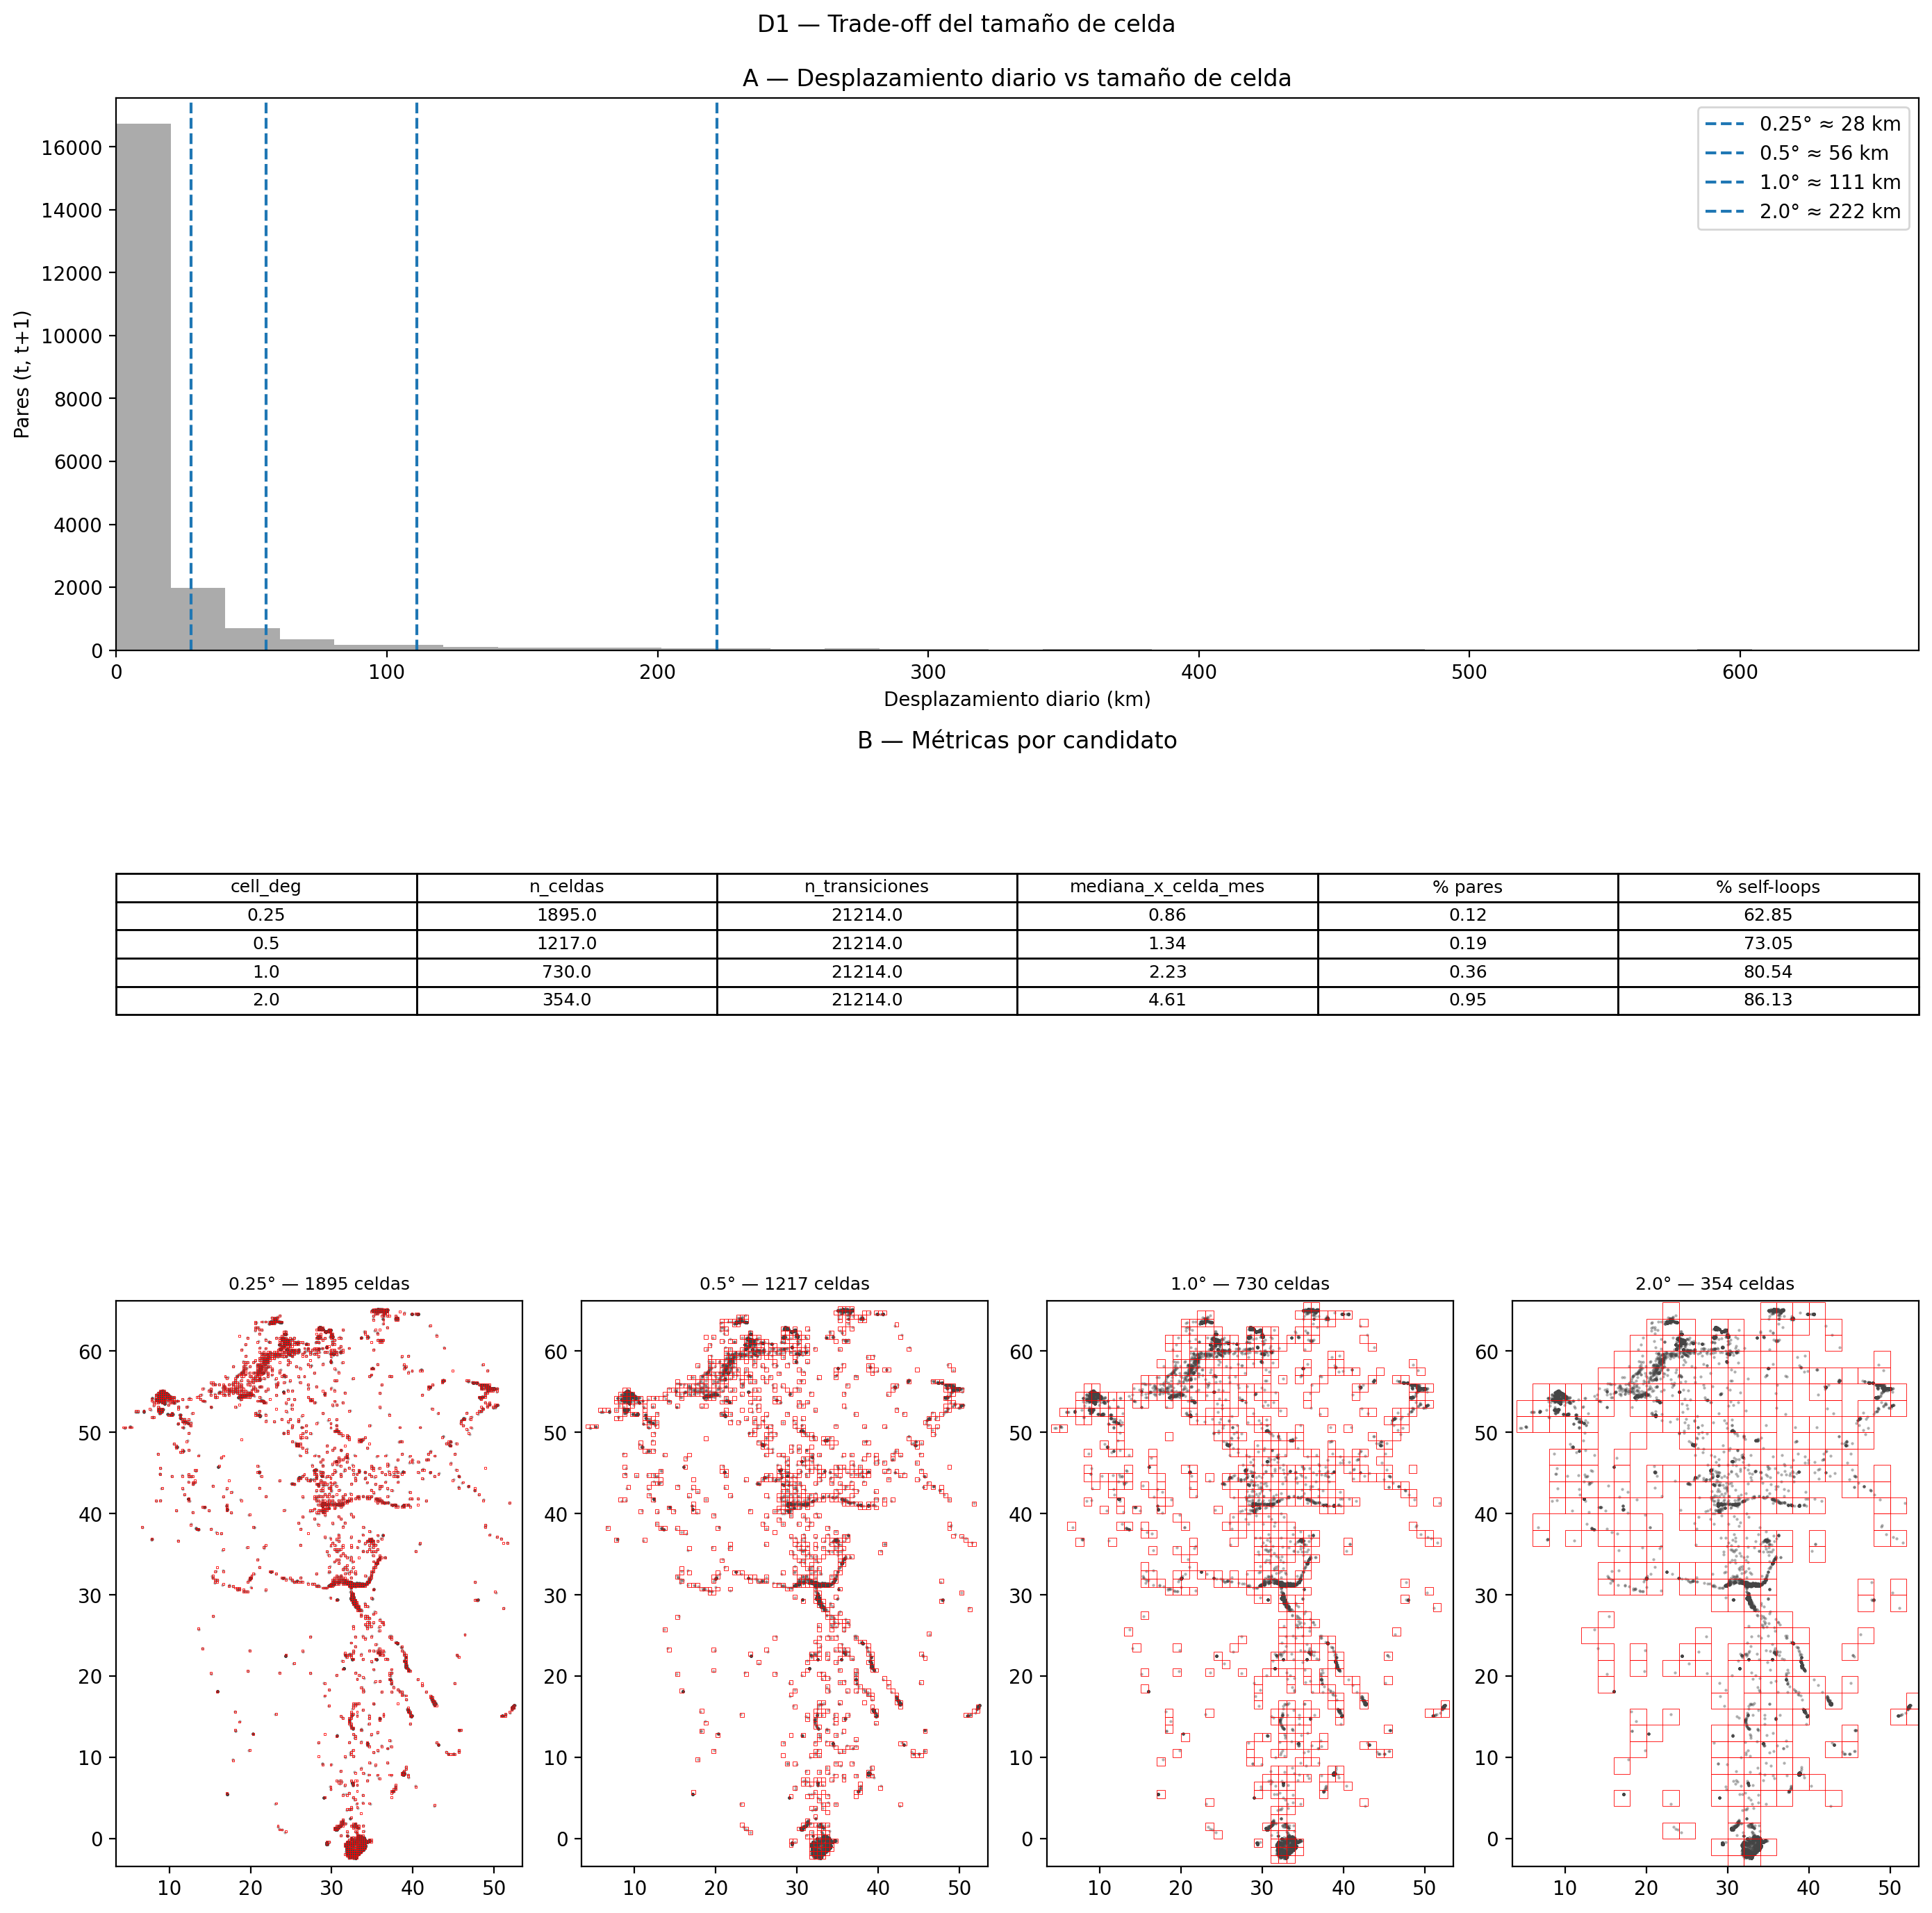
\includegraphics[width=\linewidth]{o2_fig01_grid-size-tradeoff.png}
  \caption[Compromiso del tamaño de celda]{Comparación de cuatro tamaños de celda
  para la discretización del espacio (0,25\textdegree, 0,5\textdegree, 1\textdegree\
  y 2\textdegree). Panel A: distribución del desplazamiento diario observado, con
  líneas verticales en el tamaño físico aproximado de cada celda. Panel B: métricas
  de cobertura y densidad por candidato (celdas activas, transiciones, mediana de
  transiciones por celda-mes, porcentaje de pares observados y de self-loops). Panel
  C: cada rejilla superpuesta a la nube de \textit{fixes} válidos. Se adopta
  0,5\textdegree\ porque equilibra resolución espacial y densidad estadística sin
  inflar artificialmente los self-loops.}
  \label{fig:o2-grid}
\end{figure}

\chapter{Detección de comportamiento con modelos ocultos de Markov}
\label{ch:o3}

El capítulo anterior cerró señalando dos límites de la cadena de Markov visible que
su formulación no podía salvar: no distinguía el régimen de comportamiento de cada
día (si el ave permanecía en su zona o estaba en plena migración) ni la ruta propia
de cada individuo. Este capítulo aborda el primero. La cuestión que plantea es si un
modelo no supervisado puede descubrir, en las series de posiciones diarias de
\textit{Larus fuscus}, esos regímenes que la cadena visible promediaba sin
separarlos: el movimiento de la especie alterna fases sedentarias (en las zonas de
cría e invernada) con fases de desplazamiento dirigido (los pasos migratorios de
primavera y otoño), pero el conjunto de datos no trae ninguna etiqueta que indique,
para un día concreto, en cuál de los dos regímenes se encontraba el ave. El resultado
no será todavía una predicción de la posición, sino una etiqueta de comportamiento
por ave y día.

La cadena de Markov visible no podía separar esos regímenes porque su único estado,
la celda ocupada, no distinguía si el ave permanecía en su zona o migraba. El modelo
oculto de Markov sí los separa al introducir una variable latente, el estado de
comportamiento, del que depende el movimiento de cada día. Su marco formal se expone
en el capítulo \ref{ch:preliminares} (sección \ref{sec:prelim-hmm}); aquí se ajusta un
modelo con dos estados ocultos, que se nombran \emph{estacionario} (movimiento local) y
\emph{migración} (desplazamiento dirigido de largo alcance), con la justificación de su
número en la sección \ref{sec:o3-modelo}.

El modelo es global: sus parámetros los comparten las 82 aves del conjunto. A
diferencia del capítulo anterior, donde las rutas individuales hacían que un modelo
poblacional generalizara mal a un ave no vista, aquí el estado se infiere a partir de
variables cinemáticas (la distancia recorrida y el cambio de rumbo, sección
\ref{sec:o3-features}) comparables entre individuos, sobre las que sí es razonable
compartir parámetros.

Partiendo de la misma tabla diaria del capítulo \ref{ch:o1} (una posición por ave y
día natural, con los huecos representados de forma explícita), el capítulo produce una
salida de doble uso: cada observación (ave, día) recibe una etiqueta de estado y la
probabilidad de cada régimen, que los modelos supervisados del capítulo \ref{ch:o4}
consumen como variable de entrada de alto nivel y que, a la vez, permite estratificar
por régimen el análisis del error del capítulo \ref{ch:o5}, separando el acierto de
los días sedentarios del de los días de migración. El estado detectado es la pieza que
conecta la fenología de la especie con los modelos predictivos del resto del trabajo.

\section{Variables del movimiento}
\label{sec:o3-features}

El modelo no observa la posición directamente, sino un vector de variables que resume
el movimiento de cada día y que es la observación $O_t$ que emite el estado oculto
(capítulo \ref{ch:preliminares}, ecuación \ref{eq:prelim-emision}). La elección de esas
variables determina qué puede separar el modelo: deben distinguir un día sedentario de
uno de migración a partir de la geometría de la trayectoria, no de la posición
absoluta. Se emplean dos variables cinemáticas, calculadas sobre las posiciones diarias
del capítulo \ref{ch:o1}.

La primera es el desplazamiento diario, \texttt{step\_in\_km}: la distancia de
Haversine (ecuación \ref{eq:haversine}) entre la posición de ayer y la de hoy, en
kilómetros y sin transformación. Es la señal primaria del régimen, porque separa por
sí sola los dos modos del movimiento de la especie: un día sedentario recorre unos
pocos kilómetros y uno de migración, cientos. Conservar la escala original en lugar de
comprimirla con un logaritmo es una decisión deliberada que la sección
\ref{sec:o3-modelo} justifica. La segunda es el cambio de rumbo,
\texttt{cos\_turning\_in}: el coseno del ángulo entre el rumbo de hoy (el del tramo de
ayer a hoy) y el del día anterior. Distingue la forma del movimiento: un valor próximo
a $+1$ indica rumbo sostenido (trayectoria rectilínea, propia del vuelo migratorio
dirigido), uno próximo a $-1$ una inversión de la marcha y uno próximo a $0$ un giro de
90\textdegree. Se codifica como coseno, y no como el ángulo en valor absoluto, porque
es una función suave en toda la recta que se ajusta mejor a la emisión gaussiana del
modelo, mientras que el valor absoluto introduce en el cero un quiebro que distorsiona
la distribución.

Ambas variables son entrantes: describen el tramo ya recorrido hasta el día $t$ (de
$t-1$ a $t$), no el que vendrá después (de $t$ a $t+1$). Así caracterizan el día con
información disponible en el momento y no con la posición futura, una propiedad que la
sección \ref{sec:o3-modelo} retoma al inferir el estado.

Estas dos variables forman el vector de observación de un primer modelo, el cinemático
(modelo A). Un segundo modelo (modelo B) añade tres variables de contexto ambiental y
temporal: la cobertura de vegetación baja (\texttt{veg\_low}) y alta
(\texttt{veg\_high}), tomadas de las covariables ambientales del conjunto Movebank, y
las horas de luz (\texttt{daylight\_hours}), calculadas con una fórmula astronómica a
partir de la latitud y la fecha. Estas tres variables se incorporan para tratar de
reflejar mejor la realidad biológica de los patrones migratorios, que no dependen solo
del movimiento sino también del hábitat y de la época del año. Las dos coberturas de
vegetación se mantienen separadas, porque la baja (pastos, cultivos) y la alta (bosque)
son biomas distintos que sumar en una sola variable confundiría. La comparación entre ambos modelos se resuelve en la sección
\ref{sec:o3-resultados}; hasta entonces, el que incorpora el contexto es el de
referencia.

\chapter{Predicción supervisada del movimiento diario}
\label{ch:o4}

El capítulo anterior cerró con un modelo no supervisado que separaba los dos regímenes
de comportamiento de \textit{Larus fuscus}, los días sedentarios de los de migración,
pero que no predecía dónde estaría el ave al día siguiente. Este capítulo retoma esa
pregunta, ya pendiente desde el final del capítulo \ref{ch:o2}, y la responde con
modelos supervisados que combinan tres fuentes de información: la posición diaria del
capítulo \ref{ch:o1}, la cinemática del tramo recién recorrido y la etiqueta de
régimen producida por el HMM del capítulo \ref{ch:o3}. La pregunta concreta es la
misma que en la cadena de Markov visible, dado dónde está hoy el ave, ¿dónde estará
mañana?, pero la respuesta dispone ahora de variables adicionales y de algoritmos no
lineales, y se evalúa contra los dos mismos rivales: la persistencia trivial y la
cadena de Markov de primer orden.

El capítulo plantea dos formulaciones del problema. La primera es la natural por
simetría con el capítulo de Markov, una clasificación de la celda del día siguiente
sobre la misma rejilla de 0,5\textdegree; sirve para caracterizar el techo del
enfoque y diagnosticar dónde falla. La segunda reformula el objetivo como una
regresión continua del desplazamiento diario y añade una banda de incertidumbre
interpretable, que es la salida natural para llevar la predicción a un mapa. Las dos
formulaciones se entrenan sobre las mismas variables y la misma partición temporal y
se comparan contra los mismos baselines, de modo que cualquier diferencia entre ellas
es atribuible al planteamiento del problema y no a la preparación de los datos.

El producto del capítulo, una predicción por ave y día con su banda de incertidumbre,
alimenta los mapas del capítulo \ref{ch:o5}, que cartografían el error y lo
estratifican por régimen y por mes. La preparación común a las dos formulaciones
(datos, variables, familias, métricas y baselines) se fija en la sección
\ref{sec:o4-diseno} y no se vuelve a tocar; las dos formulaciones se desarrollan en
las secciones \ref{sec:o4-categorica} y \ref{sec:o4-cuantiles}, y la
\ref{sec:o4-sintesis} consolida el techo común y deja definido lo que recibe el
capítulo siguiente.

\section{Datos, variables y diseño experimental}
\label{sec:o4-diseno}

\subsection{Entrada y partición temporal}
\label{sec:o4-datos}

Las dos formulaciones del capítulo parten de los mismos dos entregables: la tabla
diaria del capítulo \ref{ch:o1} (una posición por ave y día natural, con los huecos
representados de forma explícita) y la tabla de cinemática y régimen del capítulo
\ref{ch:o3} (la cinemática entrante de cada día, la etiqueta de estado del HMM causal
y su probabilidad asociada, más la columna \texttt{split} que asigna cada fila a
entrenamiento, validación o prueba). La partición temporal del HMM se reutiliza
intacta, sin volver a inducirla, para garantizar que el HMM y los modelos
supervisados se evalúan sobre los mismos días futuros de las mismas aves.

Sobre esa unión se construye el conjunto candidato del capítulo. Cada fila es un par
(ave, día $t$) con su día siguiente $t+1$ disponible: el día $t$ debe tener
cinemática válida del HMM, su posición y la de $t+1$ deben caer en una celda activa
de la rejilla del capítulo \ref{ch:o2}, y el día $t+1$ debe ser el día natural
inmediatamente posterior al $t$ (los pares que atraviesan un hueco calendario se
descartan, para evitar que el modelo aprenda transiciones inexistentes). El resultado
son 20\,188 pares candidatos, repartidos en 14\,598 de entrenamiento, 1\,630 de
validación interna y 3\,960 de prueba, una proporción 72/8/20 que las 82 aves
mantienen en los tres subconjuntos. Sobre estos pares se entrenan y se evalúan todos
los modelos del capítulo, supervisados y baselines, de modo que la comparación es en
igualdad estricta.

La elección de partición es deliberada. La alternativa más exigente, dejar fuera del
entrenamiento todas las observaciones de un ave (\textit{leave-one-bird-out}),
reproduce el fallo diagnosticado en el capítulo \ref{ch:o2}: en ese protocolo, una
fracción importante de los orígenes del conjunto de prueba no estaba representada en
el entrenamiento y la cadena de Markov caía a la distribución marginal del mes. La
partición temporal por ave que se adopta aquí evalúa, en cambio, el escenario
operativo del capítulo \ref{ch:o5}: predecir el futuro próximo de aves cuyo
comportamiento histórico se ha observado en el pasado. En este protocolo, la fracción
de orígenes del conjunto de prueba que el entrenamiento no ha visto baja al 10,7\,\%
(y la de destinos no vistos al 11,1\,\%), lo que sitúa al modelo en un régimen
razonable para juzgar su capacidad predictiva real, sin el sesgo pesimista del
\textit{leave-one-bird-out} ni el optimista de una partición aleatoria.

\subsection{Variables predictivas}
\label{sec:o4-features}

El modelo dispone de diez variables, que se agrupan en tres bloques. La posición
actual del ave aporta el contexto geográfico (\texttt{lat}, \texttt{lon}). El ciclo
anual se codifica con una pareja de variables cíclicas
($\sin\!\tfrac{2\pi\, \mathrm{doy}}{365}$, $\cos\!\tfrac{2\pi\, \mathrm{doy}}{365}$,
donde \textit{doy} es el día del año), que evita la discontinuidad artificial del 31
de diciembre al 1 de enero. El movimiento reciente se resume con la cinemática del
tramo entrante $t\!-\!1 \!\to\! t$ del capítulo \ref{ch:o3}, ya definida allí en sus
términos: el desplazamiento del tramo (\texttt{step\_in\_km}), su dirección codificada
como seno y coseno del rumbo (\texttt{sin\_bearing\_in}, \texttt{cos\_bearing\_in}) y
el coseno del giro respecto al tramo anterior (\texttt{cos\_turning\_in}). Y la salida
del HMM aporta el régimen como dos variables, la etiqueta de estado
(\texttt{state\_b\_causal}) y la probabilidad de migración del día
(\texttt{posterior\_b\_migracion\_causal}), ambas decodificadas por filtrado
\textit{forward-only}.

Todas las variables respetan un mismo criterio de diseño: ninguna observa el día
$t+1$ que se quiere predecir. Es un criterio firme. Una variable que dependa de la
posición de $t+1$ filtra el objetivo y produce métricas optimistas que no
corresponden al uso real del modelo, en el que el día $t+1$ aún no se ha observado.
La cinemática entrante satisface el criterio porque resume el movimiento ya
recorrido hasta el final del día $t$, la inercia real con la que el ave llega al
arranque del día siguiente; la cinemática \emph{saliente} ($t \!\to\! t\!+\!1$), en
cambio, lo violaría. La etiqueta de régimen del HMM también lo satisface por la
construcción causal del capítulo \ref{ch:o3}: el filtrado \textit{forward-only} computa
la probabilidad del estado en $t$ a partir únicamente de las observaciones hasta $t$,
sin mirar al futuro.

\subsection{Familias supervisadas y configuración}
\label{sec:o4-modelos}

El capítulo compara las tres familias de aprendizaje basadas en árboles introducidas
en el capítulo \ref{ch:preliminares}, sección \ref{sec:prelim-ml}: bosques aleatorios
\cite{breiman2001}, XGBoost \cite{chen2016} y LightGBM \cite{ke2017}. Es la
comparativa comprometida en la introducción y la que cierra la simetría con los
modelos no supervisados de los capítulos anteriores: tres algoritmos de capacidad
similar, ajustados al mismo problema, los mismos datos y la misma métrica.

Cada familia se entrena con una configuración fija y conservadora de hiperparámetros,
sin barrido por rejilla. La configuración se resume en la tabla
\ref{tab:o4-hyperparams}. El criterio es metodológico, no de comodidad: un barrido por
rejilla optimiza el rendimiento sobre el conjunto de validación interna, lo que
introduce un sesgo de selección sobre esa misma validación que infla las métricas
reportadas y dificulta separar la mejora real del azar entre configuraciones próximas.
El control del sobreajuste se delega aquí en tres mecanismos independientes: los
hiperparámetros conservadores (profundidad acotada, hojas con soporte mínimo y muestreo
estocástico de filas y columnas en \textit{boosting}), la parada temprana basada en la
validación interna (los modelos de \textit{boosting} fijan un máximo de 1\,000
iteraciones y detienen el entrenamiento si la pérdida en validación no mejora en 50
iteraciones consecutivas) y el diagnóstico explícito de la diferencia entre el error
en entrenamiento y en validación.

\begin{table}[H]
  \centering
  \small
  \begin{tabular}{lll}
    \toprule
    \textbf{Familia} & \textbf{Hiperparámetro} & \textbf{Valor} \\
    \midrule
    \multirow{3}{*}{Bosque aleatorio}
      & \texttt{n\_estimators}    & 300 \\
      & \texttt{max\_depth}       & 12 \\
      & \texttt{min\_samples\_leaf} & 10 \\
    \midrule
    \multirow{6}{*}{XGBoost}
      & \texttt{learning\_rate}   & 0,05 \\
      & \texttt{max\_depth}       & 6 \\
      & \texttt{min\_child\_weight} & 10 \\
      & \texttt{subsample}        & 0,8 \\
      & \texttt{colsample\_bytree} & 0,8 \\
      & \texttt{n\_estimators}    & 1\,000 con parada temprana a 50 \\
    \midrule
    \multirow{5}{*}{LightGBM}
      & \texttt{learning\_rate}   & 0,05 \\
      & \texttt{num\_leaves}      & 31 \\
      & \texttt{min\_child\_samples} & 20 \\
      & \texttt{subsample} / \texttt{colsample\_bytree} & 0,8 / 0,8 \\
      & \texttt{n\_estimators}    & 1\,000 con parada temprana a 50 \\
    \bottomrule
  \end{tabular}
  \caption[Configuración de hiperparámetros]{Configuración fija de hiperparámetros por
  familia, compartida por las dos formulaciones del capítulo. Los valores son
  conservadores y reflejan el consenso de la literatura aplicada para datos tabulares
  de tamaño moderado; el control del sobreajuste se delega en la combinación de la
  configuración, la parada temprana sobre la validación interna y el diagnóstico
  \textit{train-test}.}
  \label{tab:o4-hyperparams}
\end{table}

\subsection{Métricas y baselines}
\label{sec:o4-metricas}

Las métricas de evaluación son las mismas del capítulo \ref{ch:o2}, para que la
comparación entre capítulos sea directa. La proporción de aciertos en el primer
intento (\textit{top-1}) y entre los tres primeros (\textit{top-3}) mide la precisión
puntual sobre la celda; la mediana de la distancia geográfica entre el centroide de la
celda predicha y la posición real cuantifica, en kilómetros, cuánto se desvía cuando
falla. El logaritmo de la pérdida (\textit{log-loss}), heredado del cierre del capítulo de
Markov, evalúa la calidad probabilística completa de la distribución que cada modelo
entrega sobre las celdas, no sólo el acierto del primer intento, y por tanto complementa
a las métricas de precisión puntual con una dimensión que éstas no recogen. La elección
entre familias dentro de cada formulación pondera todas estas métricas en conjunto,
sin que una sola decida por sí sola: una familia con mejor \textit{log-loss} pero
distancia mediana sensiblemente peor o un sobreajuste marcado no se prefiere a una
alternativa más equilibrada. La formulación continua de la sección
\ref{sec:o4-cuantiles} no produce una distribución categórica nativa y se evalúa con
sus propias métricas geométricas allí.

El análisis del error se desagrega en cuatro cortes que se aplican a las dos
formulaciones. El \emph{global} resume el comportamiento sobre todo el conjunto de
prueba. Los cortes por régimen del HMM, \emph{estacionario} y \emph{migración},
distinguen los días en los que el ave permanece en su zona de los de desplazamiento
dirigido (3\,509 frente a 451 días en el conjunto de prueba, según
\texttt{state\_b\_causal}); separar estos dos regímenes es necesario porque una
métrica global está dominada por la moda mayoritaria del objetivo (los días
estacionarios) y oculta el comportamiento del modelo donde el problema es realmente
informativo. El cuarto corte, \emph{días de movimiento real}, selecciona los días en
los que la celda de $t+1$ difiere de la de $t$; es el escenario en el que la
persistencia trivial vale cero por construcción y donde un modelo predictivo tiene
sentido.

Los dos baselines del capítulo \ref{ch:o2} se reutilizan, reentrenados sobre la misma
partición temporal por ave para que la comparación sea en igualdad. La
\emph{persistencia} predice que mañana el ave seguirá en la celda de hoy; su
distribución es degenerada (asigna toda la masa a una celda) y no produce
\textit{log-loss} comparable, pero sigue siendo la referencia exigente que el resto
del trabajo persigue. La \emph{cadena de Markov de primer orden con estacionalidad
mensual}, ajustada sobre el conjunto de entrenamiento de este capítulo, es el rival
con distribución probabilística completa: un modelo no lineal supervisado debe, al
menos, mejorarlo para justificar su mayor complejidad.

\section{Predicción categórica de la celda}
\label{sec:o4-categorica}

La primera formulación es la natural por simetría con el capítulo \ref{ch:o2}: el
objetivo de la predicción es la celda de 0,5\textdegree{} del día siguiente, tratada
como una categoría más entre las 871 celdas activas que las posiciones del conjunto
de entrenamiento ocupan en algún momento. La rejilla y el horizonte son los mismos
que en la cadena de Markov, de modo que el \textit{top-1}, el \textit{top-3} y la
distancia mediana del modelo supervisado son directamente comparables con los de los
dos baselines. La pregunta operativa que esta sección responde no es sólo si el
supervisado bate a los baselines, sino dónde y por qué falla, porque ese diagnóstico
es el que motiva la reformulación de la sección \ref{sec:o4-cuantiles}.

\subsection{Planteamiento del problema}
\label{sec:o4-cat-planteamiento}

Cada par (ave, día~$t$) del conjunto candidato de la sección \ref{sec:o4-datos} se
convierte en un ejemplo de entrenamiento o de evaluación: la entrada son las diez
variables de la sección \ref{sec:o4-features} en el día $t$, la etiqueta es el
identificador de la celda que la posición de $t+1$ ocupa. Las tres familias de la
sección \ref{sec:o4-modelos} se ajustan en modo \emph{poblacional}: un único modelo
sobre las 82 aves, sin la identidad del individuo (\texttt{bird\_id}) entre las
variables. La decisión es deliberada y se sostiene desde dos argumentos. El primero
es de uso: el modelo poblacional cubre tanto a las aves ya observadas en
entrenamiento como a un ave nueva no vista, y no hace falta un modelo distinto por
individuo. El segundo es empírico, y se cierra en la sección
\ref{sec:o4-cat-diagnostico}: un clasificador entrenado únicamente con los datos del
ave de mayor histórico no supera al poblacional evaluado sobre las mismas
observaciones, lo que indica que la distribución poblacional ya captura la
heterogeneidad inter-individual sin necesidad de personalizar.

\subsection{Resultados globales y descarte de LightGBM}
\label{sec:o4-cat-globales}

La comparativa global sobre el conjunto de prueba se resume en la tabla
\ref{tab:o4-cat-globales} y se visualiza en la figura \ref{fig:o4-cat-modelos}. El
bosque aleatorio y XGBoost rinden de forma casi indistinguible entre sí en las
cuatro métricas y quedan en la misma banda; LightGBM, sobre los mismos datos, se
separa visiblemente por uno o dos órdenes de magnitud en \textit{log-loss} y en
distancia mediana, valores incompatibles con los de las otras dos familias.

\begin{table}[H]
  \centering
  \footnotesize
  \begin{tabular}{lrrrr}
    \toprule
    \textbf{Modelo} & \textbf{\textit{top-1}} & \textbf{\textit{top-3}} & \textbf{\textit{log-loss}} & \textbf{Dist.\,mediana (km)}\\
    \midrule
    Persistencia       & 0,778 & 0,778 &       & 20,9 \\
    Cadena de Markov   & 0,552 & 0,637 &       & 24,7 \\
    Bosque aleatorio   & 0,576 & 0,732 & 5,49  & 24,1 \\
    XGBoost            & 0,582 & 0,702 & 5,60  & 24,3 \\
    LightGBM           & 0,359 & 0,579 & 13,12 & 147,7 \\
    \bottomrule
  \end{tabular}
  \caption[Métricas globales sobre el conjunto de prueba]{Métricas globales sobre el
  conjunto de prueba (3\,960 pares (ave, día), el último 20\,\% de los días de cada
  ave). El \textit{log-loss} se computa sobre las 871 celdas activas del
  entrenamiento; los baselines no producen una distribución comparable y se dejan en
  blanco en esa columna. La distancia es la mediana entre el centroide de la celda
  predicha y la posición real. La persistencia domina las cuatro métricas
  comparables y LightGBM queda visiblemente separado por su divergencia en
  validación interna (figura \ref{fig:o4-cat-curvas}).}
  \label{tab:o4-cat-globales}
\end{table}

\begin{figure}[H]
  \centering
  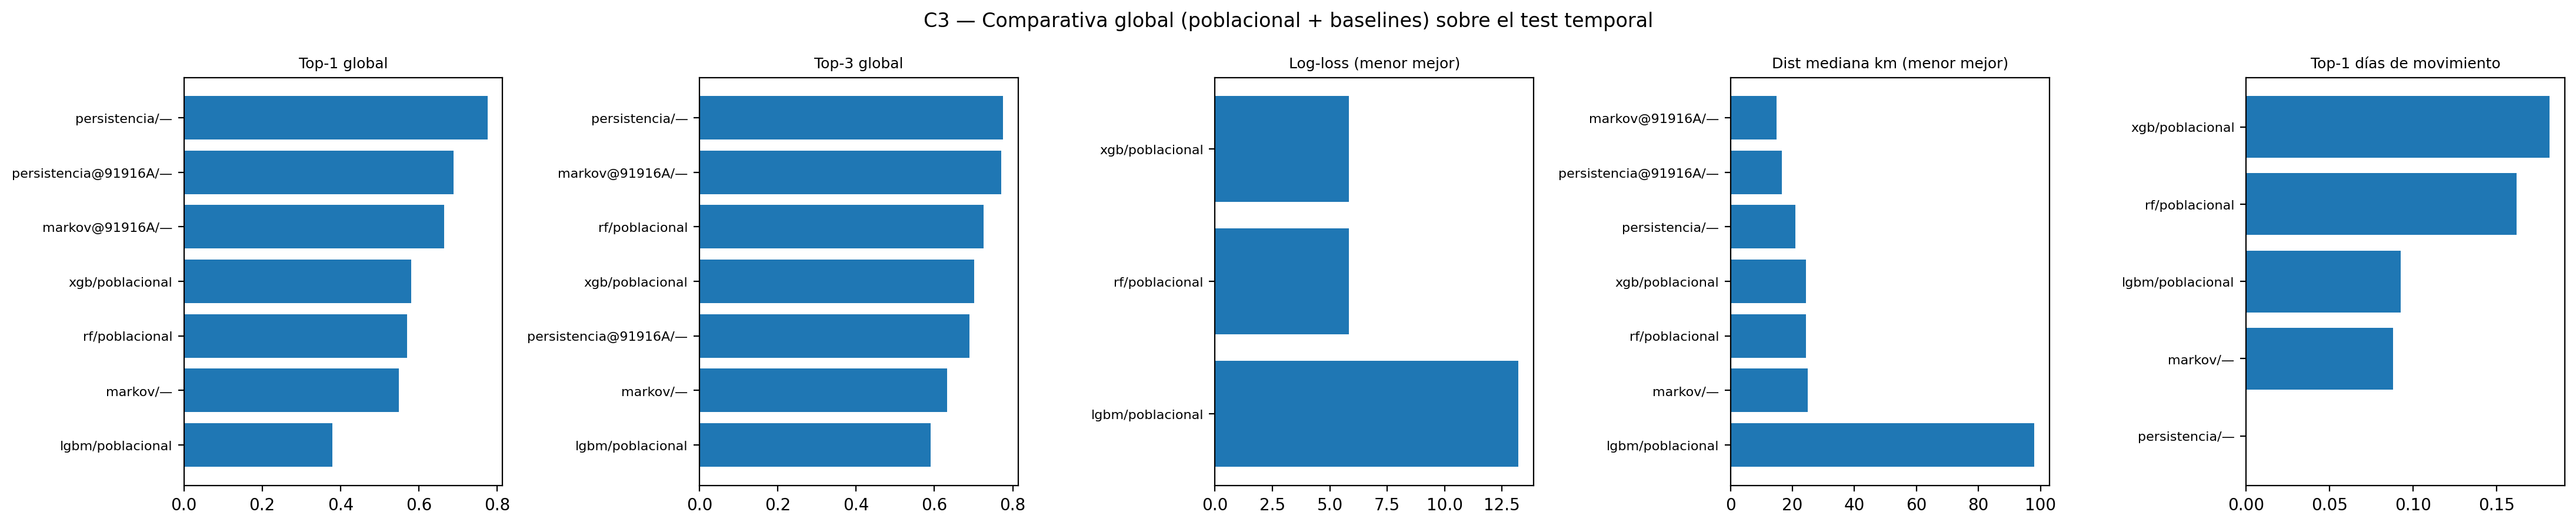
\includegraphics[width=\linewidth]{o4_fig04_models-comparison.png}
  \caption[Comparativa global de los modelos supervisados y los baselines]{Métricas
  globales sobre el conjunto de prueba (3\,960 pares (ave, día), $20\,\%$ último de
  cada ave) de las tres familias supervisadas en modo poblacional (bosque aleatorio,
  XGBoost y LightGBM) frente a los dos baselines del capítulo \ref{ch:o2}
  (persistencia y cadena de Markov de primer orden). Los cinco paneles muestran, de
  izquierda a derecha, el \textit{top-1} y el \textit{top-3} globales, la mediana de
  la distancia en kilómetros, el \textit{log-loss} sobre las 871 celdas activas y el
  \textit{top-1} restringido a los días en los que el ave cambia efectivamente de
  celda. La persistencia domina las métricas globales y LightGBM queda
  visiblemente separado por su \textit{log-loss} y su distancia anómalos, coherentes
  con la divergencia diagnosticada en la figura \ref{fig:o4-cat-curvas}.}
  \label{fig:o4-cat-modelos}
\end{figure}

La separación de LightGBM no es una variabilidad estadística sino un fallo de ajuste
diagnosticable, que la figura \ref{fig:o4-cat-curvas} expone. La curva del
\textit{log-loss} sobre la validación interna empieza ya por encima del valor que
daría una distribución uniforme sobre las 871 celdas ($\log 871 \approx 6{,}77$) y
sube de forma monótona desde la primera iteración hasta estabilizarse en torno a 32,
lo que activa la parada temprana en la iteración 1; XGBoost, sobre los mismos datos y
con un esquema de regularización análogo, desciende como cabe esperar y se detiene en
torno a la iteración 320. La interpretación es que la configuración conservadora de
LightGBM, pensada para evitar el sobreajuste sobre datos tabulares de complejidad
moderada, no extrae señal generalizable de un objetivo de muy alta cardinalidad y
distribución desbalanceada como el del problema categórico aquí planteado: con 871
clases activas en entrenamiento y un peso fuertemente desigual entre ellas, las hojas
de pequeño soporte y la división del crecimiento por hojas que caracterizan a
LightGBM no consiguen aproximar la distribución condicional, mientras que el
crecimiento por niveles y la regularización explícita de XGBoost sí lo hacen. La
familia se descarta como candidato sobre la formulación categórica; en la sección
\ref{sec:o4-cuantiles}, cuando el objetivo deja de ser categórico, vuelve a ser
viable y se reincorpora a la comparativa.

\begin{figure}[H]
  \centering
  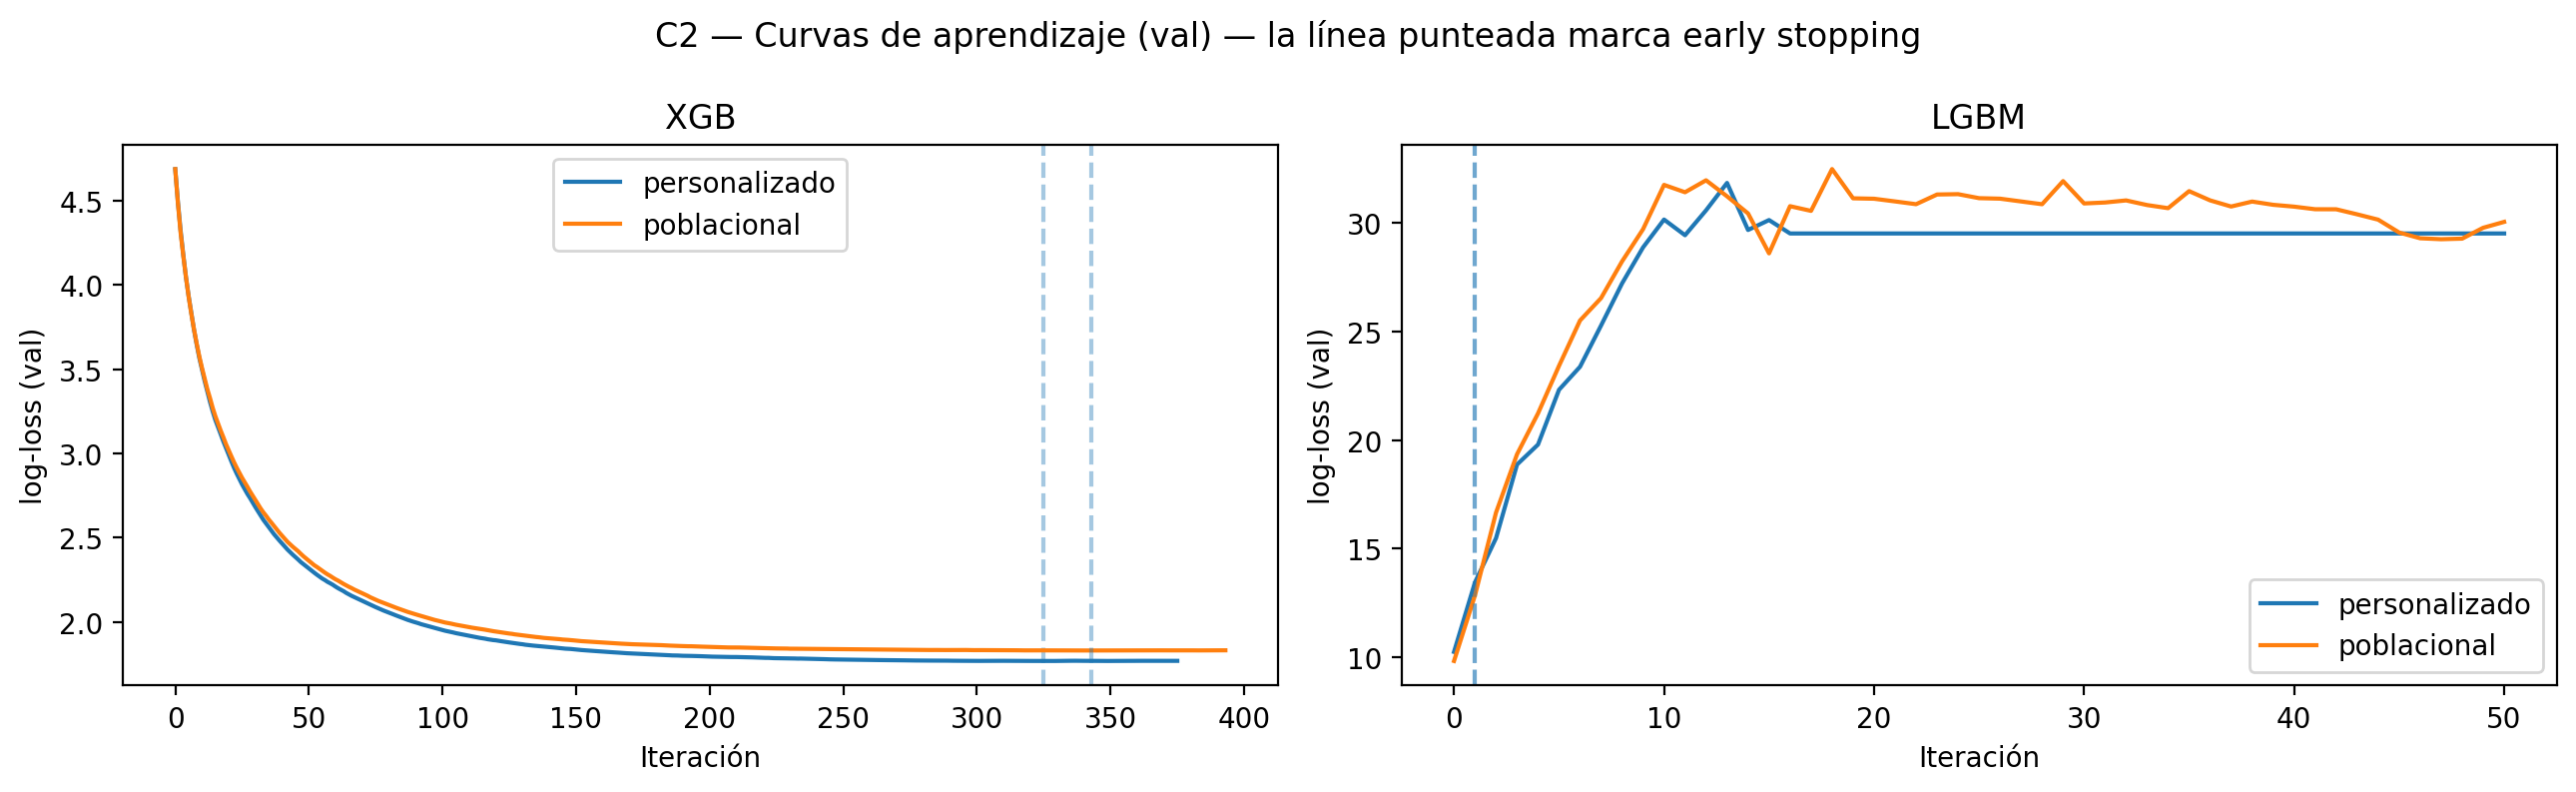
\includegraphics[width=\linewidth]{o4_fig03_learning-curves.png}
  \caption[Curvas de aprendizaje sobre la validación interna]{Evolución del
  \textit{log-loss} sobre la validación interna a lo largo de las iteraciones de
  \textit{boosting} para XGBoost (izquierda) y LightGBM (derecha), en modo
  poblacional. La línea vertical punteada marca la iteración en la que la parada
  temprana (paciencia de 50) detiene el entrenamiento. XGBoost desciende
  monótonamente hasta estabilizarse en torno a la iteración 320; LightGBM, en
  cambio, arranca ya por encima del valor de una distribución uniforme sobre las 871
  clases activas ($\log 871 \approx 6{,}77$) y crece sin pausa, lo que indica que su
  configuración conservadora no extrae señal generalizable de este objetivo
  multiclase de alta cardinalidad y distribución desbalanceada.}
  \label{fig:o4-cat-curvas}
\end{figure}

\subsection{Dónde y por qué falla el modelo}
\label{sec:o4-cat-error}

La lectura global de la tabla \ref{tab:o4-cat-globales} es asimétrica según el rival.
Frente a la cadena de Markov, las dos familias supervisadas que quedan ganan en las
tres métricas comparables (\textit{top-1}, \textit{top-3} y distancia mediana), con
una mejora modesta pero consistente que confirma que las variables del HMM y la no
linealidad del modelo aportan algo sobre la transición monoparamétrica de Markov.
Frente a la persistencia, en cambio, los dos modelos supervisados pierden en
\textit{top-1}: la persistencia, de distribución degenerada, asigna toda la masa
a una celda y su \textit{top-3} coincide siempre con su \textit{top-1}; aun así,
supera al mejor supervisado por 20 puntos en \textit{top-1}. En \textit{top-3} la
brecha se estrecha: el bosque aleatorio alcanza 0,732 frente al 0,778 de la
persistencia, una diferencia de 5 puntos frente a los 20 de \textit{top-1}.
El \textit{log-loss} del mejor supervisado (5,49) es
informativo en términos absolutos (mejor que el 6,77 de una distribución uniforme
sobre las 871 clases activas), pero la persistencia no produce distribución
comparable y no participa en esa columna.

La asimetría tiene una causa estructural directa: en el conjunto de prueba el ave
permanece en la misma celda el 77,8\,\% de los días, una moda absoluta del objetivo
que la persistencia explota por construcción y que cualquier modelo que asigne masa a
un movimiento paga proporcionalmente en \textit{top-1}. Es la geometría del problema
antes que el algoritmo. El desglose por régimen del HMM y por movimiento real, en la
tabla \ref{tab:o4-cat-estado} y en la figura \ref{fig:o4-cat-estado}, refina esta
lectura.

\begin{table}[H]
  \centering
  \footnotesize
  \begin{tabular}{lcccccc}
    \toprule
     & \multicolumn{2}{c}{\textbf{Estacionario}} & \multicolumn{2}{c}{\textbf{Migración}} & \multicolumn{2}{c}{\textbf{Movim.~real}}\\
     & \multicolumn{2}{c}{$n=3\,509$} & \multicolumn{2}{c}{$n=451$} & \multicolumn{2}{c}{$n=880$}\\
    \cmidrule(lr){2-3}\cmidrule(lr){4-5}\cmidrule(lr){6-7}
    \textbf{Modelo} & \textit{top-1} & \textit{top-3} & \textit{top-1} & \textit{top-3} & \textit{top-1} & \textit{top-3}\\
    \midrule
    Persistencia       & 0,841 & 0,841 & 0,284 & 0,284 & 0,000 & 0,000 \\
    Cadena de Markov   & 0,607 & 0,694 & 0,120 & 0,195 & 0,089 & 0,373 \\
    Bosque aleatorio   & 0,632 & 0,792 & 0,137 & 0,259 & 0,164 & 0,445 \\
    XGBoost            & 0,639 & 0,762 & 0,140 & 0,235 & 0,175 & 0,445 \\
    \bottomrule
  \end{tabular}
  \caption[Acierto \textit{top-1} y \textit{top-3} desagregados por régimen del HMM y por movimiento
  real]{Acierto (\textit{top-1} y \textit{top-3}) sobre el
  conjunto de prueba, desagregados por el régimen del HMM causal (\emph{estacionario}
  y \emph{migración}, según \texttt{state\_b\_causal} del capítulo \ref{ch:o3}) y
  restringidos a los días en que la celda de $t+1$ difiere de la de $t$
  (\emph{movim.~real}). Se omite LightGBM, descartado en la sección anterior.
  La persistencia, de distribución degenerada, iguala siempre su \textit{top-1} y
  su \textit{top-3}. Los modelos supervisados reducen notablemente la brecha con
  la persistencia al pasar a \textit{top-3}, y en los días de movimiento real
  la superan con claridad (0,445 frente a 0,000).}
  \label{tab:o4-cat-estado}
\end{table}

\begin{figure}[H]
  \centering
  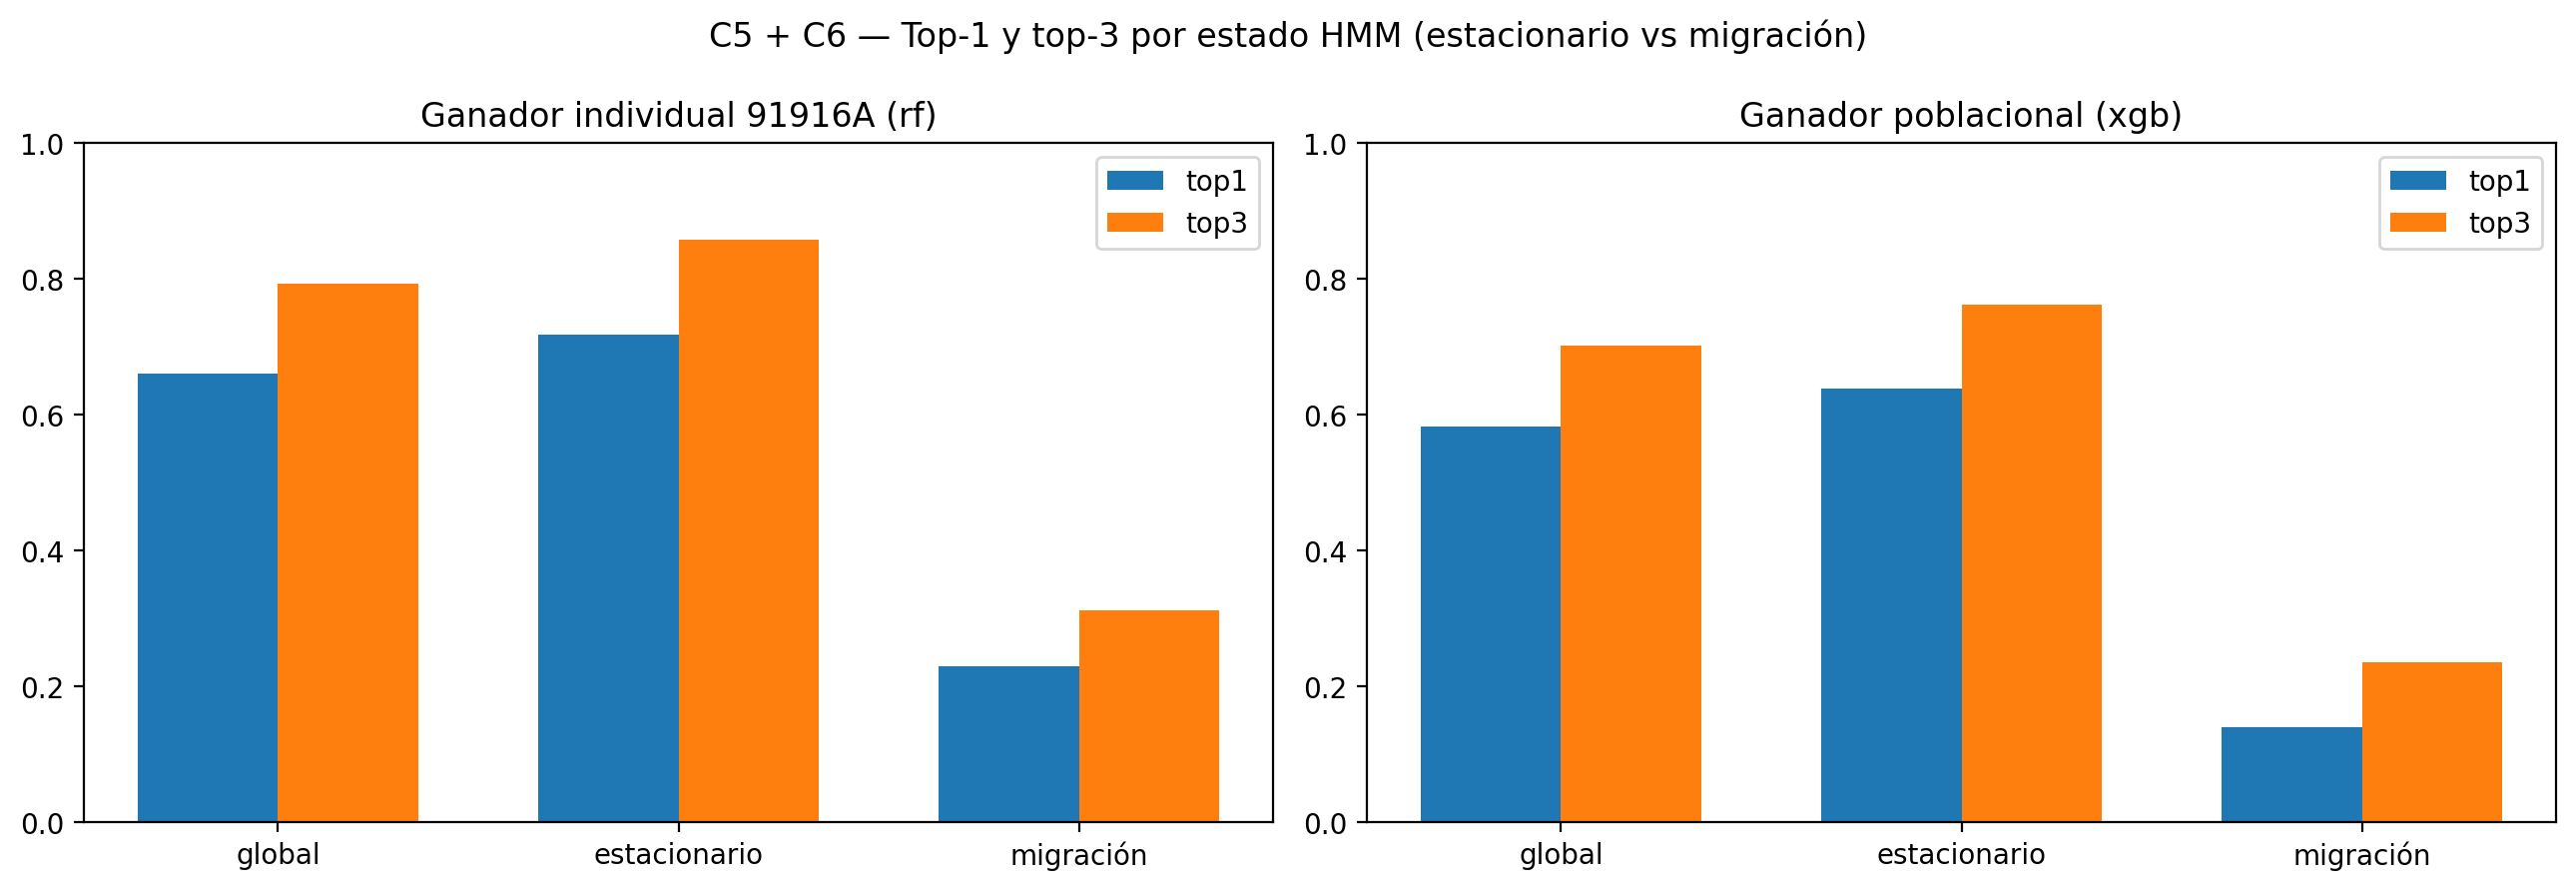
\includegraphics[width=\linewidth]{o4_fig07_error-by-state-poblacional.png}
  \caption[\textit{Top-1} y \textit{top-3} desagregados por régimen del HMM]{Acierto
  (\textit{top-1} y \textit{top-3}) del modelo poblacional (XGBoost, derecha) y del
  modelo individual del ave 91916A (bosque aleatorio, izquierda) desagregados por el
  régimen del HMM causal del capítulo \ref{ch:o3}, en el conjunto de prueba. El
  régimen \emph{estacionario} cubre 3\,509 días (88,6\,\% del conjunto) y el régimen
  \emph{migración}, 451 días (11,4\,\%). Para el poblacional, el \textit{top-1} cae de
  0,64 en estacionario a 0,14 en migración; el \textit{top-3} cae de 0,76 a 0,24.
  La brecha con la persistencia es mayor en \textit{top-1} que en \textit{top-3}, y
  se concentra en los días de migración (tabla \ref{tab:o4-cat-estado}).}
  \label{fig:o4-cat-estado}
\end{figure}

Dos lecturas. La primera, la propia caída en migración: el \textit{top-1} de los
supervisados se desploma de 0,64 a 0,14 entre los dos regímenes, y la distancia
mediana cuando fallan se dispara de 23 a más de 150\,km. Los días informativos para
la predicción son la minoría y son precisamente donde el modelo pierde casi toda su
capacidad predictiva. La segunda, que la persistencia bate al supervisado también
dentro del régimen de migración del HMM, podría parecer contradictoria con la
motivación de incorporar el régimen como variable, pero es coherente con la
definición causal del estado: la etiqueta \texttt{state\_b\_causal} se asigna a
partir del paso \emph{entrante} ($t\!-\!1 \to t$), de modo que un día puede
pertenecer al régimen de migración por haber llegado tras un desplazamiento grande,
sin que el ave haya iniciado otro desplazamiento durante $t$ ni vaya a iniciarlo en
$t+1$. En esos días, una fracción importante de los 451 marcados como migración, la
persistencia sigue acertando.

El espacio donde un modelo predictivo aporta algo que la persistencia no puede dar
por construcción es, por tanto, el de los \emph{días de movimiento real}: los 880
días del conjunto de prueba en los que la celda de $t+1$ difiere de la de $t$
(el 22,2\,\% del total). Allí la persistencia acierta cero en \textit{top-1} y
en \textit{top-3} por construcción; los modelos supervisados aciertan entre 0,16 y
0,18 en \textit{top-1} y llegan a 0,445 en \textit{top-3}, frente al 0,373 de la
cadena de Markov. El margen es modesto en \textit{top-1}, pero en \textit{top-3}
los supervisados superan claramente a Markov y aplican sobre la persistencia una
ventaja que este contexto permite cuantificar; es el único corte en el que ambas
comparaciones resultan favorables al modelo supervisado.

\subsection{De dónde sale la señal}
\label{sec:o4-cat-importancia}

La descomposición por importancia relativa de las variables, en la figura
\ref{fig:o4-cat-importancia}, ordena cuantitativamente las tres fuentes de
información de las que dispone el modelo. La posición acapara la mayor parte: la
latitud y la longitud suman 0,75 de la importancia normalizada en el modelo
poblacional, lo que reproduce numéricamente la dominación del régimen estacionario
detectada en la sección anterior. El bloque de variables del HMM contribuye 0,05
(la probabilidad de migración) más 0,03 (la etiqueta de estado), una suma modesta
pero coherente: el aporte del HMM al modelo supervisado pasa principalmente por la
\emph{probabilidad blanda} del régimen, que matiza el comportamiento del clasificador
en la franja ambigua entre los días claramente estacionarios y los claramente
migratorios, mientras que la \emph{etiqueta dura} del estado, que en su mayor parte
sólo replica información ya recogida en la probabilidad, pesa poco más de la mitad que
aquella y no llega a ser determinante. El bloque del ciclo anual (seno y coseno del
día del año) suma 0,09 y la cinemática entrante (desplazamiento, rumbo y giro)
alrededor de 0,09. Las variables del HMM, por tanto, están en el mismo orden de
magnitud que el ciclo anual y la cinemática: aportan señal real al supervisado,
modesta y principalmente a través del posterior blando.

\begin{figure}[H]
  \centering
  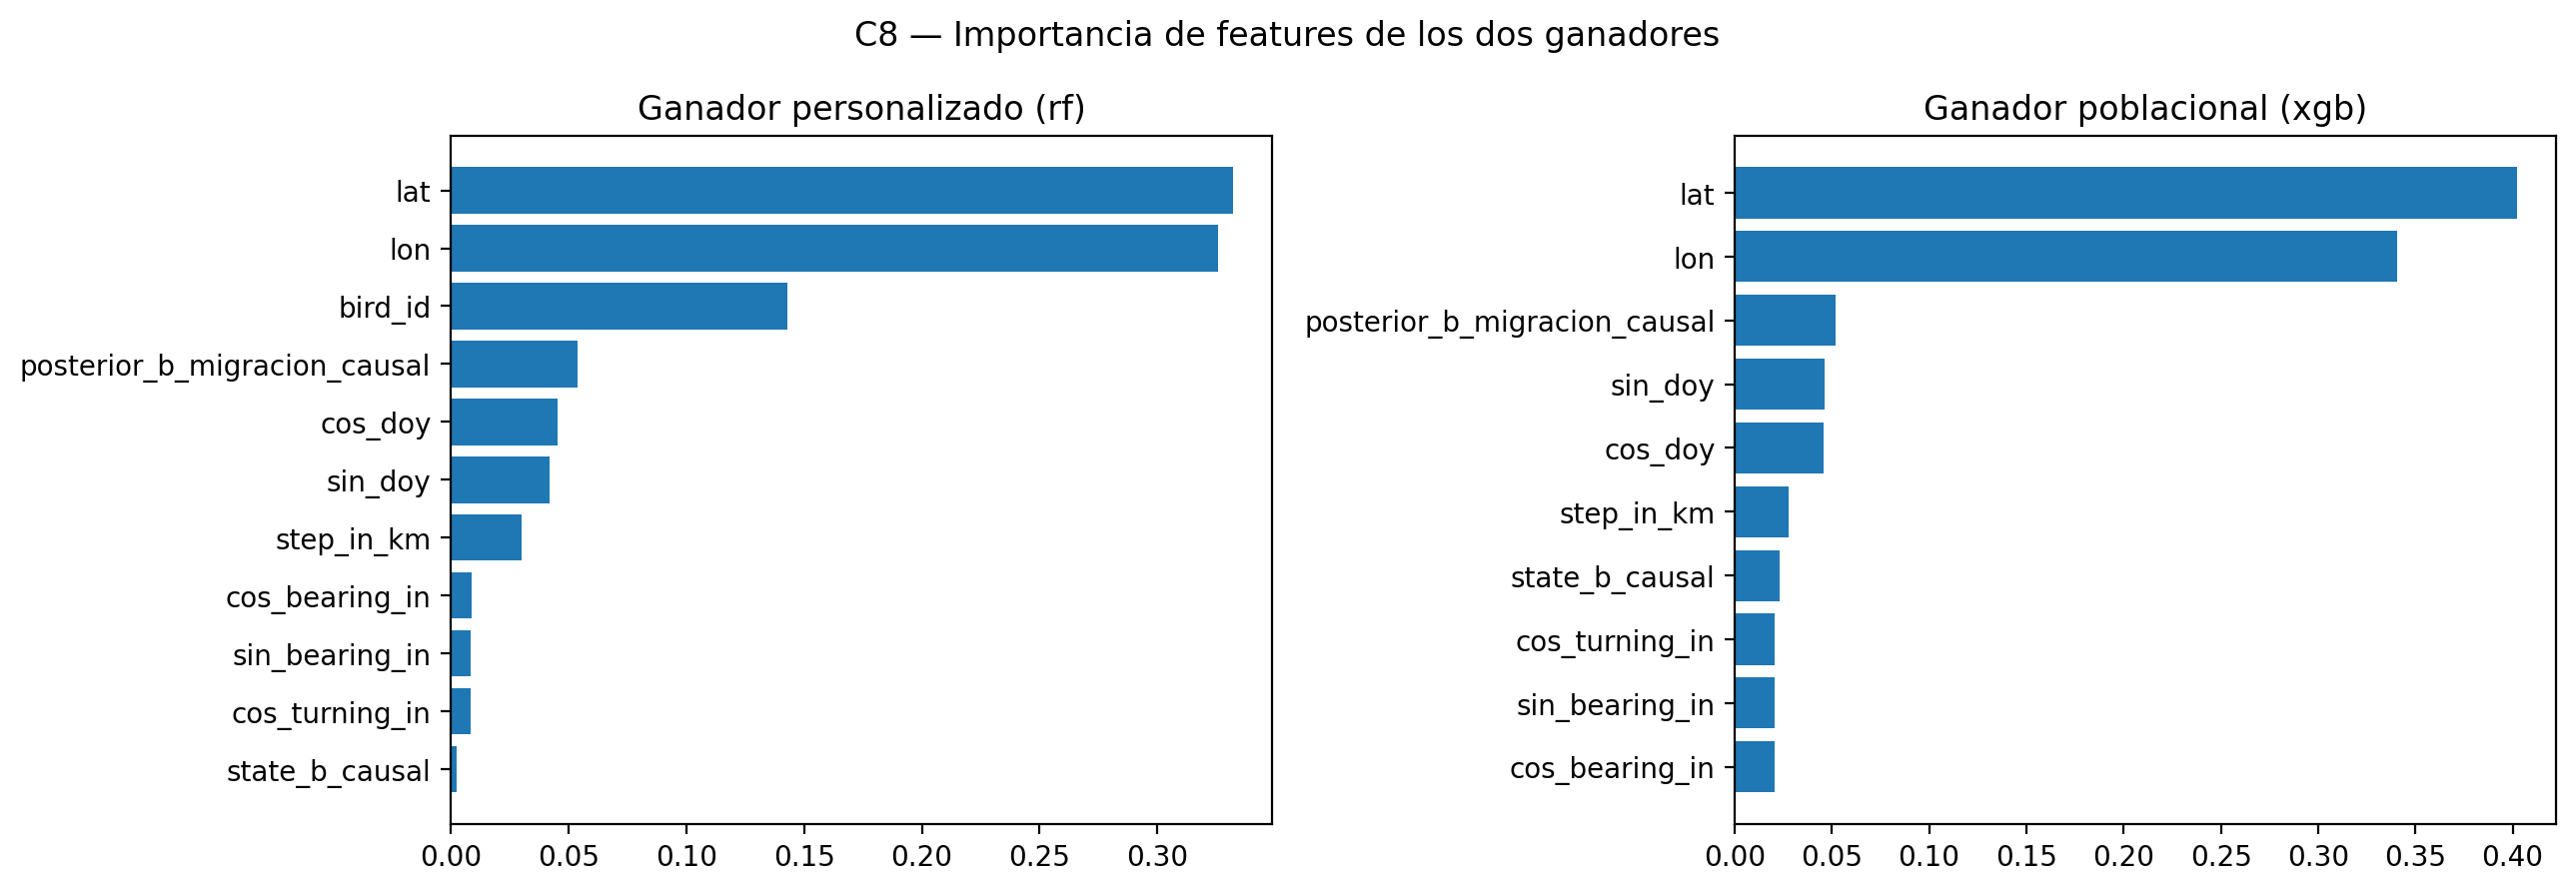
\includegraphics[width=\linewidth]{o4_fig09_feature-importance-winners.png}
  \caption[Importancia relativa de las variables]{Importancia relativa de las diez
  variables predictivas para el modelo poblacional (XGBoost, izquierda) y para el
  bosque aleatorio entrenado únicamente con el ave 91916A (derecha; ver
  \ref{sec:o4-cat-diagnostico}). En ambos casos la posición (latitud y longitud)
  acapara la mayor parte de la importancia (0,75 en el poblacional, 0,63 en el
  modelo individual). Las variables del HMM aportan 0,05 (probabilidad de migración)
  más 0,03 (etiqueta de estado) en el modelo poblacional y suben a 0,13 más 0,004
  en el modelo individual, donde la señal geográfica se reduce y el régimen blando
  pasa a tener un peso mayor. La etiqueta dura del estado pesa siempre menos que la
  probabilidad blanda; el aporte del HMM al supervisado pasa principalmente por esta última.}
  \label{fig:o4-cat-importancia}
\end{figure}

\subsection{Diagnóstico del techo y cierre del alcance}
\label{sec:o4-cat-diagnostico}

La formulación categórica permite, por tanto, situar dos causas estructurales del
techo de rendimiento que las dos secciones siguientes recogen. La primera es que el
objetivo categórico desperdicia la geometría del espacio: un error que predice una
celda vecina (un desplazamiento de unas decenas de kilómetros) se penaliza
exactamente igual que un error que predice una celda en el otro extremo del dominio
(varios miles), y el modelo no recibe ninguna información sobre la distancia entre
clases en su función de pérdida. Bajo esta restricción, los días de movimiento real
quedan condenados a un \textit{top-1} bajo, porque acertar la celda exacta de
destino es un problema más estricto que predecir la dirección y la magnitud del
desplazamiento. La sección \ref{sec:o4-cuantiles} reformula el objetivo justamente
para devolverle al modelo la información geométrica que la formulación categórica
descarta. La segunda causa es de horizonte y de variables: a un día con variables
locales (posición, cinemática del tramo entrante, ciclo anual y régimen del HMM) le
falta el predictor causal de un evento migratorio (la disponibilidad de vientos
favorables, la historia multi-día del desplazamiento, el destino al que el ave se
dirige), y ninguna combinación de algoritmo y arquitectura puede inventar lo que las
variables no contienen. Esta segunda causa es común a las dos formulaciones del
capítulo y se argumenta de forma cuantitativa, ya con los resultados de ambas a la
vista, en la sección \ref{sec:o4-sintesis}.

Un último apunte sobre el alcance del entrenamiento cierra esta sección y deja
zanjada la elección poblacional anunciada en la sección
\ref{sec:o4-cat-planteamiento}. Un bosque aleatorio entrenado únicamente con los
1\,458 días de entrenamiento del ave de mayor histórico (91916A) y evaluado sobre
sus 406 días de prueba alcanza un \textit{top-1} de 0,660 y un \textit{log-loss} de
4,33; el modelo poblacional restringido a las mismas 406 observaciones obtiene
\textit{top-1} 0,653 y \textit{log-loss} 2,72, prácticamente igual en acierto y
sensiblemente mejor en calidad probabilística. La heterogeneidad inter-individual
que el capítulo \ref{ch:o1} anticipaba y el capítulo \ref{ch:o3} cuantificaba existe,
pero la distribución poblacional ya la captura tan bien como un modelo dedicado al
individuo con más datos posible, sin la complejidad ni la falta de escalabilidad de
entrenar un modelo por ave. La formulación continua de la sección siguiente confirma
este resultado con un experimento análogo y diferente, y la sección
\ref{sec:o4-sintesis} consolida el cierre.

\section{Predicción continua del desplazamiento con cuantiles}
\label{sec:o4-cuantiles}

Esta sección desarrolla una respuesta de modelado a la primera de las dos causas
del techo diagnosticadas en la sección \ref{sec:o4-cat-diagnostico}, la que es
salvable sin cambiar el horizonte ni las variables: reformular el problema como una
regresión del desplazamiento diario en lugar de una clasificación de la celda. Con
las mismas variables, la misma partición temporal y los mismos hiperparámetros
conservadores, la reformulación devuelve al modelo la información geométrica del
espacio que la formulación categórica descartaba (el acierto \textit{top-1} sube 18
puntos a nivel global y la distancia mediana del error en los días de migración del
HMM se reduce a un tercio) y, al estimarse en forma de cuantiles, entrega además
una predicción que sale del modelo como un punto del plano acompañado de un
intervalo $[p_{10}, p_{90}]$ por componente, una banda de incertidumbre
interpretable que la clasificación no podía dar y que el capítulo \ref{ch:o5} lleva
al mapa.

\subsection{Reformulación del objetivo y arquitectura del modelo}
\label{sec:o4-q-planteamiento}

El objetivo de la predicción deja de ser el identificador discreto de la celda y
pasa a ser el desplazamiento del ave entre dos días consecutivos, expresado en
grados: $\Delta\mathrm{lat} = \mathrm{lat}(t\!+\!1) - \mathrm{lat}(t)$ y
$\Delta\mathrm{lon} = \mathrm{lon}(t\!+\!1) - \mathrm{lon}(t)$. La elección de la
parametrización cartesiana frente a la polar (distancia, rumbo) es deliberada y
evita la discontinuidad angular en $\pm 180^\circ$, que rompería la suavidad del
objetivo para los pasos de orientación este-oeste y obligaría a un tratamiento
especial. Las dos componentes se predicen por separado y de forma independiente, con
un modelo por componente.

Para acompañar cada predicción puntual de una banda de incertidumbre se ajustan, para
cada componente, tres cuantiles condicionales en lugar de la media: $p_{10}$, $p_{50}$
y $p_{90}$. La estimación minimiza la pérdida cuantílica
(capítulo \ref{ch:preliminares}, sección \ref{sec:prelim-cuantil},
ecuación \ref{eq:prelim-pinball}), que penaliza de forma asimétrica los errores por
exceso y por defecto según el cuantil buscado y, en su agregado sobre los tres
cuantiles, permite ajustar simultáneamente la mediana condicional $p_{50}$ (la
predicción puntual del desplazamiento) y los dos extremos del intervalo
$[p_{10}, p_{90}]$ (una banda de incertidumbre con cobertura nominal del 80\,\%). La
monotonía $p_{10} \leq p_{50} \leq p_{90}$ no la garantiza el ajuste cuando cada
cuantil se estima con un modelo independiente y se fuerza, cuando es necesario, por
ordenación a posteriori; la fracción de filas afectadas y las diferencias entre
familias se analizan en la sección \ref{sec:o4-q-incertidumbre}.

Las tres familias del capítulo se comparan también en esta formulación. XGBoost y
LightGBM minimizan directamente la pérdida cuantílica para cada cuantil, mientras
que el bosque aleatorio, cuyos árboles parten por reducción de la varianza y no
optimizan directamente esa pérdida, obtiene los cuantiles \emph{a posteriori} como
cuantiles empíricos de la distribución de los valores del objetivo en cada hoja, en
la formulación de bosque de regresión cuantílica de \cite{meinshausen2006}. La
ablación per-individuo, que en la formulación categórica se ensayó con un bosque
aleatorio entrenado únicamente con el ave de mayor histórico, se repite aquí con
XGBoost y se comenta en la sección \ref{sec:o4-q-cierre}.

Para comparar con la formulación categórica de la sección \ref{sec:o4-categorica} y
con los baselines, la predicción puntual $p_{50}$ se discretiza al \textit{grid} de
0,5\textdegree{} (un \textit{top-1 mapeado} que cuenta como acierto las
predicciones cuyo punto cae en la celda real) y la distancia se reporta tanto
\emph{nativa} (la distancia entre el punto predicho y la posición real, sin
discretizar) como \emph{vía centroide} (entre el centroide de la celda en la que cae
el punto predicho y la posición real, comparable con la distancia mediana de la
sección \ref{sec:o4-categorica}).

\subsection{La mejora respecto a la formulación categórica}
\label{sec:o4-q-precision}

La tabla \ref{tab:o4-q-precision} pone lado a lado el mejor modelo de la sección
\ref{sec:o4-categorica} (XGBoost categórico), las tres familias de la regresión de
cuantiles y la persistencia trivial sobre el conjunto de prueba, desagregados por
régimen del HMM y por movimiento real. La figura \ref{fig:o4-q-distancia} visualiza
la distribución completa de la distancia entre el punto predicho y la posición
real para las tres familias de cuantiles.

\begin{table}[H]
  \centering
  \footnotesize
  \begin{tabular}{lcccccccc}
    \toprule
     & \multicolumn{2}{c}{\textbf{Global}} & \multicolumn{2}{c}{\textbf{Estacionario}} & \multicolumn{2}{c}{\textbf{Migración}} & \multicolumn{2}{c}{\textbf{Movim.~real}}\\
     & \multicolumn{2}{c}{$n=3\,960$} & \multicolumn{2}{c}{$n=3\,509$} & \multicolumn{2}{c}{$n=451$} & \multicolumn{2}{c}{$n=880$}\\
    \cmidrule(lr){2-3}\cmidrule(lr){4-5}\cmidrule(lr){6-7}\cmidrule(lr){8-9}
    \textbf{Modelo} & \textit{top-1} & \textit{top-3} & \textit{top-1} & \textit{top-3} & \textit{top-1} & \textit{top-3} & \textit{top-1} & \textit{top-3}\\
    \midrule
    \multicolumn{9}{l}{\emph{Formulación categórica (sección \ref{sec:o4-categorica}, referencia)}}\\
    XGBoost categórico  & 0,582 & 0,702 & 0,639 & 0,762 & 0,140 & 0,235 & 0,175 & 0,445 \\
    \midrule
    \multicolumn{9}{l}{\emph{Formulación continua (esta sección)}}\\
    Bosque aleatorio    & 0,771 & 0,898 & 0,842 & 0,946 & 0,217 & 0,523 & 0,049 & 0,566 \\
    XGBoost             & 0,763 & 0,901 & 0,833 & 0,946 & 0,217 & 0,552 & 0,100 & 0,582 \\
    LightGBM            & 0,762 & 0,900 & 0,835 & 0,946 & 0,197 & 0,543 & 0,085 & 0,578 \\
    \midrule
    \multicolumn{9}{l}{\emph{Baseline}}\\
    Persistencia        & 0,778 & 0,778 & 0,841 & 0,841 & 0,284 & 0,284 & 0,000 & 0,000 \\
    \bottomrule
  \end{tabular}
  \caption[Comparativa entre las dos formulaciones del capítulo y los baselines]{Acierto
  (\textit{top-1} y \textit{top-3}, mapeados al \textit{grid} 0,5\textdegree) sobre el
  conjunto de prueba, para el mejor modelo de la formulación categórica, las tres familias
  de la regresión de cuantiles (modo poblacional) y la persistencia trivial. La predicción
  puntual de la formulación continua es el $p_{50}$ de cada componente, llevado al
  \textit{grid} 0,5\textdegree{} para comparar con la formulación categórica. La
  reformulación sube el \textit{top-1} global de 0,58 a 0,76--0,77 y el \textit{top-3}
  de 0,70 a 0,90, superando en esta última métrica a la persistencia (0,778). En los días
  de migración del HMM, el \textit{top-3} pasa de 0,24 a 0,55, el doble del baseline
  trivial. Entre familias, las tres son prácticamente indistinguibles en los cuatro cortes.}
  \label{tab:o4-q-precision}
\end{table}

\begin{figure}[H]
  \centering
  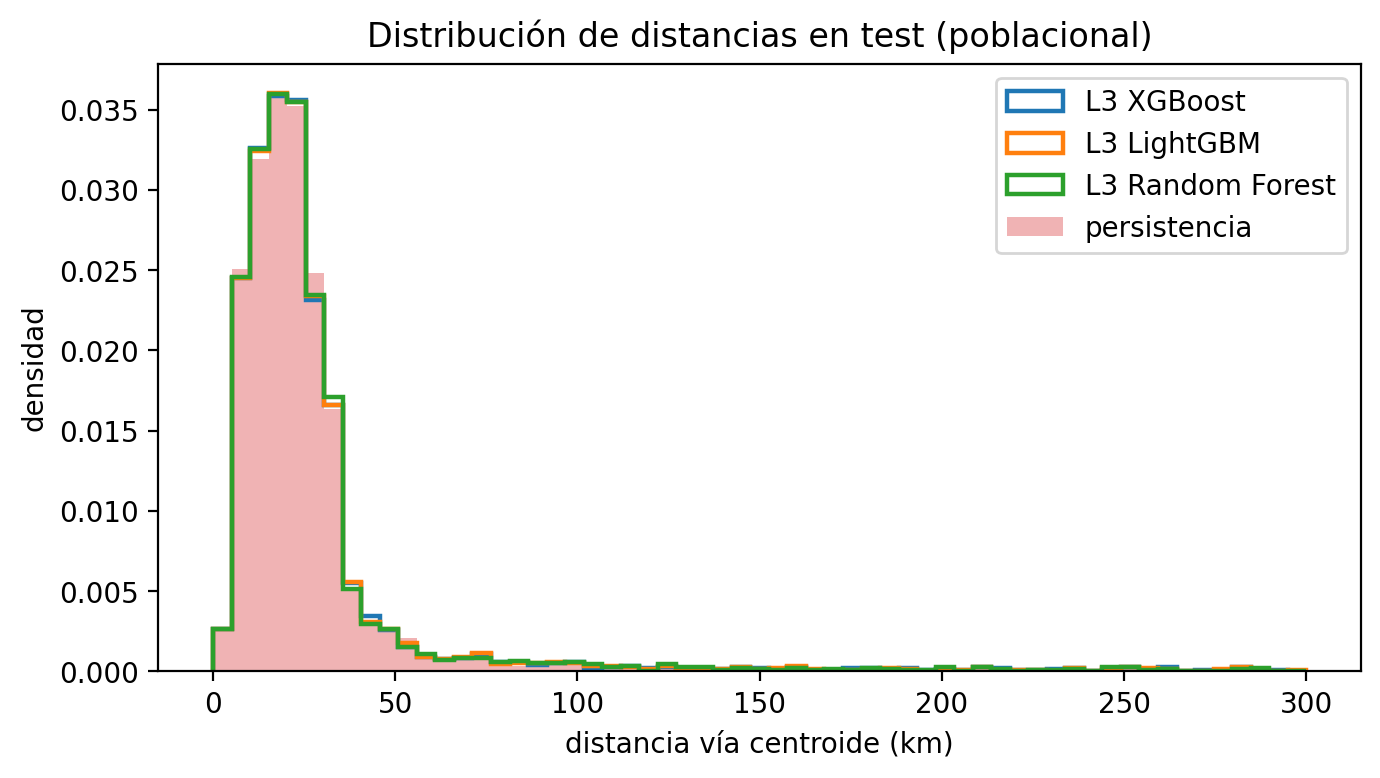
\includegraphics[width=\linewidth]{o4_fig26_distance-distribution.png}
  \caption[Distribución de la distancia entre el punto predicho y la posición
  real]{Distribución de la distancia vía centroide entre la predicción puntual
  ($p_{50}$) y la posición real, sobre el conjunto de prueba, para las tres
  familias de la regresión de cuantiles y la persistencia trivial (modo
  poblacional). Las distribuciones coinciden en el grueso (la masa concentrada por
  debajo de los 50\,km, atribuible a los días estacionarios) y se separan en la cola
  (los días de movimiento real). La diferencia entre las tres familias supervisadas
  es pequeña a lo largo de toda la distribución.}
  \label{fig:o4-q-distancia}
\end{figure}

El primer mensaje de la tabla es la magnitud de la mejora respecto a la formulación
categórica. La sola reformulación del objetivo, con las mismas variables, el mismo
\textit{split} y los mismos hiperparámetros, levanta el \textit{top-1} global de
0,58 a 0,76 (18 puntos absolutos, un 31\,\% relativo). En \textit{top-3} la mejora
es más pronunciada aún: de 0,70 a 0,90 globalmente, con lo que la formulación
continua supera ya a la persistencia (0,778) en esta métrica. En los días de
migración del HMM, el \textit{top-3} pasa de 0,24 a 0,55, el doble del nivel de
la persistencia (0,28). La mejora se reproduce en los días estacionarios
(\textit{top-1} de 0,64 a 0,83--0,84; \textit{top-3} de 0,76 a 0,946). El
mecanismo es geométrico: como el desplazamiento real es
\emph{nulo} el 77,8\,\% de los días de prueba, el regresor aprende a predecir un
desplazamiento próximo a cero en esos días, su $p_{50}$ recae en la celda de
origen y reproduce el acierto de los \textit{self-loops} que la formulación
categórica no fijaba con su argmax sobre 871 clases. Más en general, la pérdida
cuantílica penaliza el error en distancia (no por igual a todas las clases
incorrectas) y empuja al modelo hacia predicciones geométricamente cercanas, que es
exactamente lo que el problema requiere. La única métrica que se mueve a la baja en
la transición es el \textit{top-1} del corte de movimiento real (de 0,18 a 0,05--
0,10), una contrapartida coherente con el mismo mecanismo (el regresor «se atreve»
menos a apostar fuera de la celda de origen), que la ganancia en \textit{top-3}
(0,58 frente a 0,445 de la formulación categórica) compensa con holgura.

El segundo mensaje es la convergencia entre familias. Sobre el conjunto de prueba el
\textit{top-1} global queda entre 0,762 (LightGBM) y 0,771 (bosque aleatorio), una
banda de menos de un punto, con la distancia mediana indistinguible (20,9\,km en
las tres). El mismo patrón se repite en los cuatro cortes de la
tabla \ref{tab:o4-q-precision} y en la figura \ref{fig:o4-q-distancia}, donde las
tres distribuciones se superponen tanto en el grueso como en la cola. Bajo la
formulación continua, la elección de familia es secundaria para la precisión: tres
algoritmos con mecanismos distintos (\textit{bagging} no paramétrico en el bosque
aleatorio, \textit{boosting} de árboles por niveles en XGBoost y \textit{boosting}
por hojas en LightGBM) llegan al mismo lugar.

Como consecuencia secundaria de la convergencia, LightGBM no diverge aquí. La misma
familia que en la sección \ref{sec:o4-cat-globales} se separó del resto y se
descartó como candidato sobre el problema multiclase de 871 clases activas, sobre
la regresión de cuantiles (con seis modelos, uno por cuantil y eje, en lugar de un
único multiclase de muy alta cardinalidad) se ajusta sin patología y rinde
indistinguiblemente del bosque aleatorio y de XGBoost. La división del crecimiento
por hojas y el soporte mínimo conservador no extraen señal generalizable de un
objetivo de 871 clases con peso fuertemente desigual, pero sí de seis regresiones
cuantílicas escalares cada una. La familia se reincorpora a la comparativa de esta
sección en igualdad con las otras dos, y la elección del modelo recomendado para
los mapas se argumenta en la sección \ref{sec:o4-q-cierre} desde la calidad
probabilística, no desde la precisión.

Frente a la persistencia trivial, la formulación continua se sitúa en una posición
muy distinta a la categórica. Aquélla perdía en todas las métricas globales por un
margen amplio; ésta queda apenas una o dos décimas por debajo en \textit{top-1}
global y, en \textit{top-3}, supera ya a la persistencia (0,90 frente a 0,778).
En los días de migración del HMM, el \textit{top-3} de la formulación continua
(0,55) dobla al de la persistencia (0,28): la formulación aprende que en migración
el ave puede desplazarse a cualquiera de varias celdas vecinas, y distribuye masa
sobre ese vecindario de forma que las tres candidatas más probables ya superan
claramente al único destino que la persistencia propone. La persistencia conserva
una pequeña ventaja en \textit{top-1} por la moda dominante de los \textit{self-loops},
pero la diferencia deja de ser cualitativa: la formulación continua iguala o supera
a la referencia exigente del capítulo según la métrica y el corte, mientras añade
una dimensión que la persistencia no entrega, la banda de incertidumbre que la
sección \ref{sec:o4-q-incertidumbre} caracteriza.

\subsection{Banda de incertidumbre y monotonía de los cuantiles}
\label{sec:o4-q-incertidumbre}

La precisión de la predicción puntual es sólo una de las dimensiones que la
formulación de cuantiles entrega. La otra, ausente por completo en la formulación
categórica, es la \emph{incertidumbre calibrada}: para cada predicción, los
extremos $p_{10}$ y $p_{90}$ delimitan un intervalo que se espera contenga la
posición real el 80\,\% del tiempo si la calibración es correcta. La tabla
\ref{tab:o4-q-incertidumbre} resume las tres métricas que evalúan esta dimensión y
la figura \ref{fig:o4-q-calibracion} la visualiza para la cobertura.

\begin{table}[H]
  \centering
  \footnotesize
  \begin{tabular}{lcccc}
    \toprule
    \textbf{Modelo} & \textbf{Cobertura lat / lon} & \textbf{\textit{Pinball} lat / lon} & \textbf{Cruces de cuantil} \\
    \midrule
    Bosque aleatorio  & 0,862 / 0,859 & 0,081 / 0,062 & 0 \\
    XGBoost           & 0,849 / 0,840 & 0,081 / 0,063 & 54 \\
    LightGBM          & 0,836 / 0,788 & 0,079 / 0,062 & 202 \\
    \bottomrule
  \end{tabular}
  \caption[Calidad probabilística de las tres familias]{Métricas de calidad
  probabilística sobre el conjunto de prueba (3\,960 pares, modo poblacional).
  \emph{Cobertura}: fracción empírica de filas en las que la posición real cae
  dentro del intervalo $[p_{10}, p_{90}]$ predicho, por eje (objetivo nominal del
  80\,\%). \emph{Pinball}: pérdida cuantílica promedio sobre los tres cuantiles, por
  eje. \emph{Cruces de cuantil}: número de filas en las que la ordenación
  $p_{10} \leq p_{50} \leq p_{90}$ no se respetaba antes de la corrección a
  posteriori. Las tres familias tienen una \textit{pinball} prácticamente igual; se
  diferencian en la calibración (LightGBM es el más cercano al nominal) y en la
  coherencia interna de los cuantiles (el bosque aleatorio no cruza por
  construcción).}
  \label{tab:o4-q-incertidumbre}
\end{table}

\begin{figure}[H]
  \centering
  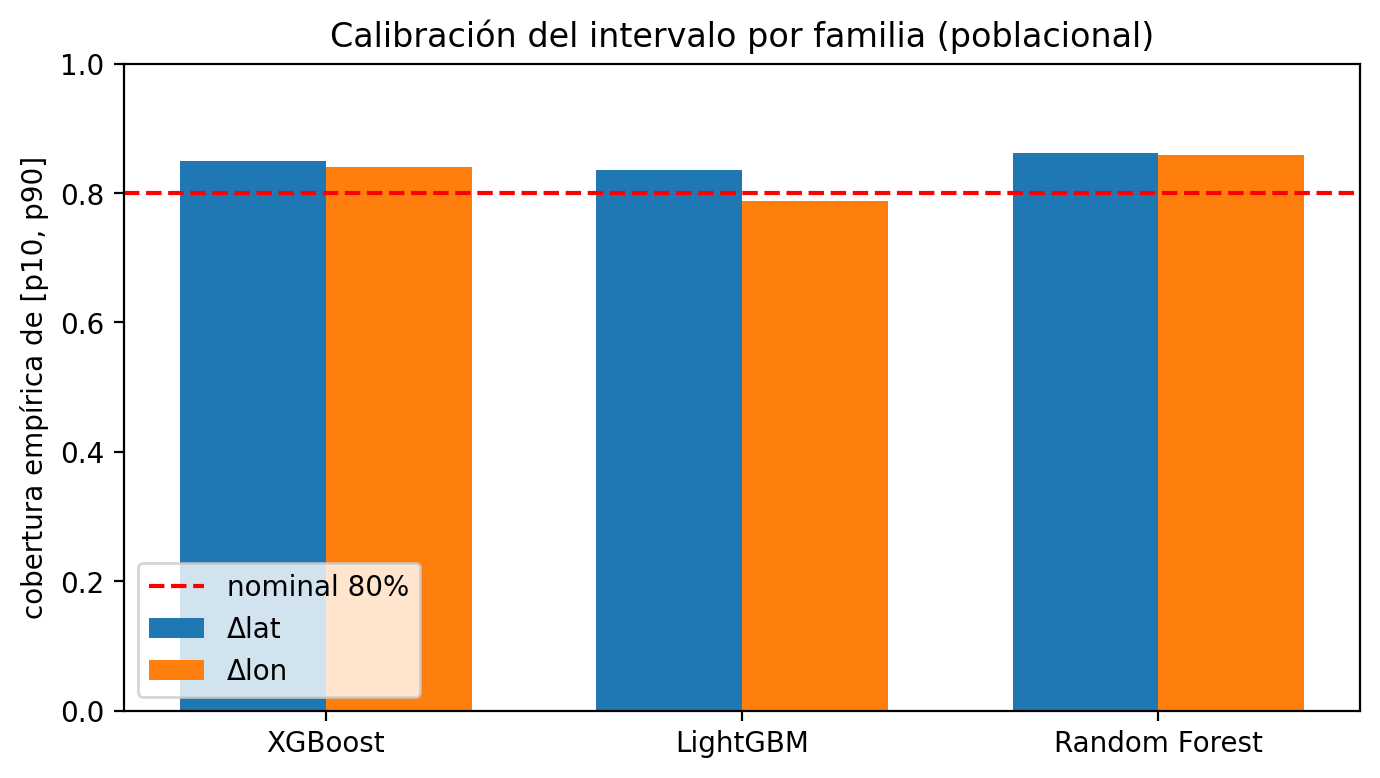
\includegraphics[width=\linewidth]{o4_fig25_calibration-coverage.png}
  \caption[Cobertura empírica del intervalo de predicción]{Cobertura empírica del
  intervalo $[p_{10}, p_{90}]$ frente al objetivo nominal del 80\,\%, por familia y
  por eje, sobre el conjunto de prueba en modo poblacional. Una cobertura próxima al
  80\,\% indica una banda de incertidumbre bien calibrada. LightGBM queda más cerca
  del nominal (con una ligera infracobertura en longitud), XGBoost se sitúa unos
  puntos por encima y el bosque aleatorio sobrecubre, con bandas más anchas en
  ambas direcciones.}
  \label{fig:o4-q-calibracion}
\end{figure}

Las tres familias comparten una pérdida cuantílica prácticamente idéntica (en torno
a 0,08 para la latitud y 0,06 para la longitud), lo que confirma que el ajuste de
los tres cuantiles es de calidad equivalente en la métrica que el problema
optimiza, pero se separan en las dos métricas que la métrica de ajuste no captura
directamente: la calibración empírica del intervalo y la coherencia interna de los
cuantiles. LightGBM queda más cerca del 80\,\% nominal (0,84 y 0,79), XGBoost se
sitúa unos puntos por encima (0,85 y 0,84) y el bosque aleatorio sobrecubre (0,86 y
0,86), con bandas más anchas que las otras dos. La interpretación es directa: el
bosque aleatorio entrega una incertidumbre conservadora, en el sentido de que su
intervalo contiene la posición real con más frecuencia de la que dice, mientras que
LightGBM la entrega más ajustada al nivel anunciado.

La columna de cruces de cuantil refleja una diferencia estructural entre las
familias, no un detalle de implementación. XGBoost y LightGBM ajustan un modelo
independiente por cuantil y por eje, y nada en su entrenamiento garantiza que la
ordenación $p_{10} \leq p_{50} \leq p_{90}$ se respete para todas las observaciones,
de modo que aparecen 54 cruces en XGBoost y 202 en LightGBM, corregibles a
posteriori por simple ordenación pero no eliminables \emph{a priori}. El bosque
aleatorio de cuantiles, en cambio, extrae los tres cuantiles de la misma
distribución empírica de cada hoja, y la ordenación se respeta por construcción:
cero cruces. Es una propiedad estructural del \textit{bagging} no paramétrico en
este problema, no una mejora de ajuste.

\subsection{Balance, alcance del entrenamiento y modelo recomendado}
\label{sec:o4-q-cierre}

El balance de la formulación continua es claro respecto a las dos referencias del
capítulo. Frente a la formulación categórica de la sección \ref{sec:o4-categorica},
la mejora es sustancial y se reproduce en todos los cortes: el \textit{top-1} global
sube 18 puntos y el \textit{top-3} global sube 20 puntos (de 0,70 a 0,90). Frente
a la persistencia trivial, la formulación continua revierte por completo la pérdida
amplia que la formulación categórica acumulaba: en \textit{top-1} queda una o dos
décimas por debajo, y en \textit{top-3} la supera (0,90 frente a 0,778 global;
0,55 frente a 0,28 en los días de migración del HMM). A ello añade la dimensión
que la persistencia no puede dar: una banda de incertidumbre calibrada $[p_{10},
p_{90}]$ con cobertura empírica próxima al 80\,\% nominal
(sección \ref{sec:o4-q-incertidumbre}). Sobre los mapas del capítulo
\ref{ch:o5}, esa banda se traduce en una región geográfica interpretable que
ninguna de las alternativas anteriores podía producir.

La elección del modelo recomendado para los mapas del capítulo siguiente pondera
las tres dimensiones que la tabla \ref{tab:o4-q-precision} y la tabla
\ref{tab:o4-q-incertidumbre} resumen, sin que ninguna decida en solitario. En
precisión las tres familias son indistinguibles, así que la decisión se traslada a
la calidad probabilística: LightGBM es el más cercano al 80\,\% nominal de
cobertura, XGBoost queda como alternativa equivalente con un margen pequeño de
sobrecobertura, y el bosque aleatorio entrega bandas perceptiblemente más anchas
con una garantía estructural de monotonía de los cuantiles. Para los mapas del
capítulo \ref{ch:o5}, el modelo recomendado es la regresión de cuantiles con
LightGBM, por entregar la banda mejor calibrada al nivel anunciado, con XGBoost
como alternativa equivalente.

Un último apunte sobre el alcance del entrenamiento, paralelo al que cierra la
sección \ref{sec:o4-cat-diagnostico}, confirma la decisión poblacional. Un regresor
de cuantiles de XGBoost entrenado únicamente con los 1\,458 días de entrenamiento
del ave de mayor histórico (91916A) y evaluado sobre sus 406 días de prueba alcanza
un \textit{top-1 mapeado} de 0,685 y una distancia mediana vía centroide de
14,6\,km; el modelo poblacional restringido a las mismas 406 observaciones obtiene
\textit{top-1} 0,687 y distancia mediana 14,4\,km, indistinguible del individual en
ambas métricas. Dos experimentos con diseños distintos (una clasificación categórica
en la sección \ref{sec:o4-cat-diagnostico} y una regresión de cuantiles aquí)
convergen, por tanto, en la misma conclusión: la distribución poblacional ya captura
al individuo más favorable tan bien como un modelo dedicado, y la heterogeneidad
inter-individual del conjunto, real, no justifica el coste de entrenar un modelo por
ave ni la pérdida de escalabilidad a las 80 aves con menos histórico. El modelo
canónico del capítulo, en sus dos formulaciones, es el poblacional.

\section{Síntesis y límites del enfoque}
\label{sec:o4-sintesis}

El capítulo ha planteado dos formulaciones del mismo problema de predicción del
movimiento diario y las ha comparado contra los dos baselines heredados del
capítulo \ref{ch:o2}. La formulación categórica caracteriza el techo del enfoque y
diagnostica sus causas; la formulación continua corrige la limitación geométrica de
la primera y entrega, además, una banda de incertidumbre interpretable. En las dos,
el modelo canónico es el poblacional: las pruebas con un clasificador y un regresor
entrenados únicamente con el ave de mayor histórico convergen en la misma
conclusión y cierran la decisión global vs per-individuo que el capítulo
\ref{ch:o1} dejó sembrada y el capítulo \ref{ch:o3} arrastró.

Las dos formulaciones convergen también en un mismo límite, que el capítulo no
puede salvar y que merece nombrarse con precisión: la predicción a un horizonte de
un día con variables locales no contiene el predictor causal de un evento
migratorio (la disponibilidad de vientos favorables, la historia multi-día del
desplazamiento, el destino al que el ave se dirige). No es una limitación del
algoritmo (la convergencia entre las tres familias sobre la regresión de cuantiles
de la sección \ref{sec:o4-q-precision} lo confirma) ni de la formulación del
objetivo (la regresión continua recupera ya la información geométrica que la
clasificación descartaba): es del planteamiento del problema a esta escala. El
trabajo futuro que se deriva es el de incorporar esas tres piezas (las variables de
viento ECMWF descartadas en el capítulo \ref{ch:o1}, la historia multi-día como
secuencia de entrada y una noción explícita del destino), todas fuera del alcance
temporal del trabajo.

El producto que el capítulo entrega al capítulo \ref{ch:o5} es la predicción del
modelo recomendado (la regresión de cuantiles con LightGBM en modo poblacional, con
XGBoost como alternativa equivalente) sobre el conjunto de prueba: para cada par
(ave, día) un punto $(\mathrm{lat}_t + p_{50,\mathrm{lat}}, \mathrm{lon}_t +
p_{50,\mathrm{lon}})$, un intervalo $[p_{10}, p_{90}]$ por componente con cobertura
empírica próxima al 80\,\% nominal, y la etiqueta de régimen del HMM causal del
capítulo \ref{ch:o3}. Los mapas del capítulo siguiente cartografían sobre esos tres
elementos el error de la predicción y lo estratifican por régimen y por mes, lo que
cierra la cadena Markov $\to$ HMM $\to$ predicción supervisada con la
visualización del comportamiento del modelo allí donde el error existe y allí donde
no.

\chapter{Visualización del movimiento en mapas interactivos}
\label{ch:o5}

El capítulo anterior entregó, para cada par (ave, día) del conjunto de prueba, una
predicción continua del movimiento del día siguiente, con un punto central y una banda
de incertidumbre por componente. Este capítulo describe la herramienta que lleva esa
predicción al mapa: un módulo de visualización que representa sobre el territorio las
rutas de las aves y su predicción, y que permite explorar de forma interactiva, en
kilómetros y de un vistazo, el error de cada predicción. La herramienta no entrena
ningún modelo nuevo ni reabre el análisis cuantitativo del error, ya realizado en el
capítulo \ref{ch:o4}; su aportación es hacer ese comportamiento tangible y explorable,
y con ella se cierra la cadena que recorre la memoria, de la cadena de Markov visible al
modelo oculto y de este a la predicción supervisada. Las secciones siguientes describen
qué ofrece la herramienta y cómo se usa, y después, brevemente, cómo se ha construido.

\section{Funcionalidades y uso}
\label{sec:o5-funcionalidades}

La herramienta es una aplicación web interactiva (figura \ref{fig:o5-app}) que se abre
directamente en el navegador, sin instalación ni servidor, y que representa sobre el mapa
el recorrido real y la predicción del modelo para cualquiera de las ochenta y dos aves
del conjunto de prueba. Toma como base la predicción recomendada del capítulo
\ref{ch:o4} y reúne en un único panel lateral las funcionalidades de exploración que se
resumen a continuación:

\begin{itemize}
  \item \textbf{Selección de ave.} Cualquiera de las aves del conjunto, ordenadas por
  histórico, más una vista «Todas» que dibuja a la vez las rutas reales de todas ellas
  (un color por ave, con resalte al pasar el ratón y acceso a la vista individual al
  pulsar sobre una de las rutas).
  \item \textbf{Predicción del día y error en kilómetros.} Para el ave elegida se
  superponen su posición real, el punto predicho a un día y su banda de incertidumbre
  $[p_{10}, p_{90}]$; una lectura destacada muestra el error de ese día en kilómetros,
  esto es, la distancia entre la predicción y la posición real. Esta lectura cumple
  directamente el cometido de analizar visualmente el error de predicción.
  \item \textbf{Reproducción temporal.} Una ventana de días (con inicio y fin
  ajustables) y los controles habituales de reproducir, pausar, avanzar o retroceder un
  día y regular la velocidad; al reproducir, la estela de la predicción va creciendo
  sobre el mapa.
  \item \textbf{Capas conmutables.} La trayectoria real completa del ave (coloreada por
  año), el punto del baseline de Markov de primer orden con su propio error, y el estado
  de comportamiento del modelo oculto del capítulo \ref{ch:o3} (estacionario o
  migración).
\end{itemize}

El uso típico es inmediato: se abre el fichero en el navegador, se elige un ave, se
ajusta la ventana de días y se pulsa reproducir para seguir, día a día, cómo la
predicción persigue a la posición real, leyendo en todo momento el error en kilómetros.
Para que esa lectura no sea ambigua, la herramienta fija un código de color estable, con
el error siempre en rojo, la posición real en verde y la predicción en granate. La misma
herramienta incluye, además, una demostración de predicción encadenada a varios pasos,
etiquetada como ilustrativa por las razones de calibración que se explican más adelante.

\begin{figure}[H]
  \centering
  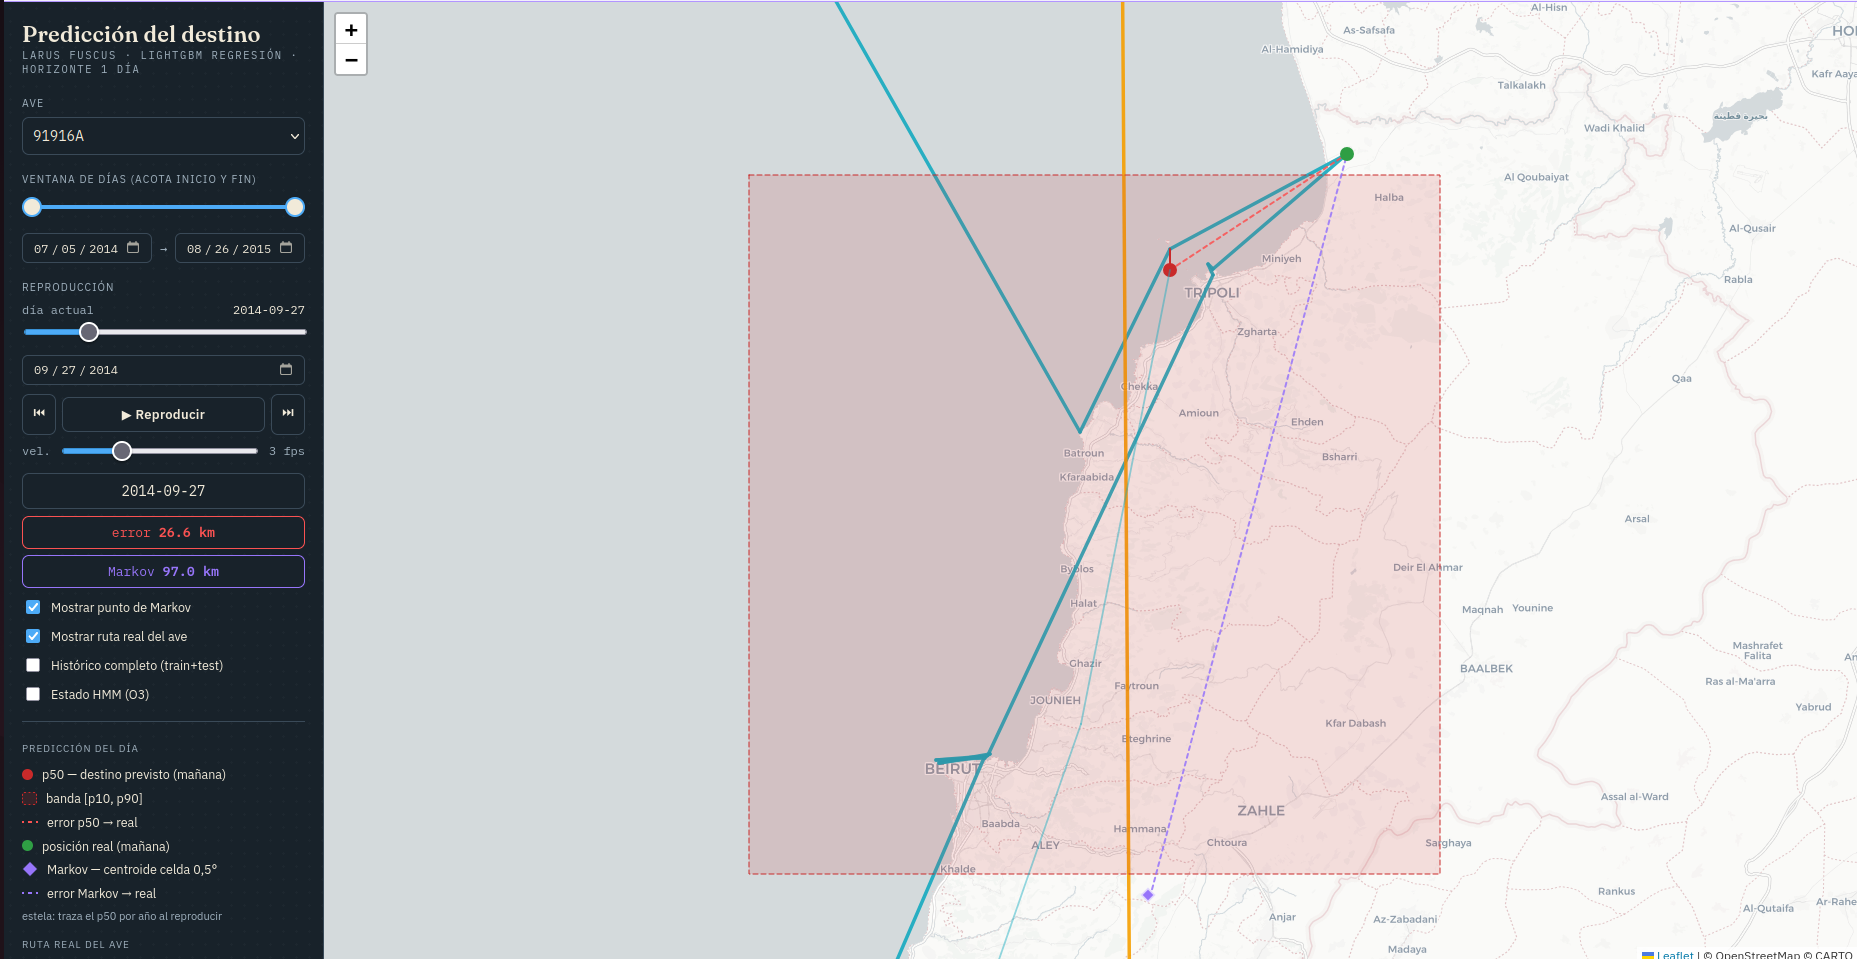
\includegraphics[width=\linewidth]{o5_prediccion_app.png}
  \caption[Aplicación interactiva de visualización de la predicción]{Captura de la
  aplicación interactiva a medida. El panel lateral reúne la selección de ave, la
  ventana y los controles de reproducción y los conmutadores de capas; el mapa muestra,
  para el día actual, la posición real, la predicción a un día con su banda de
  incertidumbre y la lectura del error en kilómetros. El fichero es una página web
  autónoma, de la que aquí se reproduce una captura estática.}
  \label{fig:o5-app}
\end{figure}

\section{Desarrollo}
\label{sec:o5-desarrollo}

El módulo se implementa en el paquete \texttt{tfg\_aves.viz}, con el mismo patrón que el
resto del trabajo: el cálculo de los agregados, en módulos de cómputo puro, se separa
del renderizado. La aplicación es una plantilla HTML que contiene todo el código de la
interfaz (estilos y lógica de cliente, sobre la biblioteca de mapas Leaflet) y en la que
se inyecta, como datos embebidos en formato JSON, la predicción de cada ave; que sea una
página estática sin servidor es posible porque las predicciones del conjunto de prueba
están precalculadas.

Sobre qué datos se dibujan se toman tres decisiones técnicas. La herramienta cartografía
el predictor recomendado por el capítulo \ref{ch:o4} (la regresión de cuantiles con
LightGBM en modo poblacional). La incertidumbre se dibuja como
el rectángulo $[p_{10}, p_{90}]$ de cada eje, y no como una elipse, porque es la
representación fiel de unos cuantiles estimados por componente. Y el horizonte de la
vista es de un solo día, el único en el que la banda está calibrada; el encadenamiento a
varios pasos se ofrece únicamente como la demostración ilustrativa ya mencionada.

% ===========================================================================
% PENDIENTE (no redactar hasta aprobación de las secciones anteriores):
%   \section{Síntesis ...}   -> cierre breve: qué hace evidente la herramienta,
%                               límites, enganche con conclusiones.
% ===========================================================================

\chapter{Análisis de impacto}
\label{ch:impacto}

De los contextos en los que un trabajo puede tener repercusión (personal,
empresarial, social, económico, medioambiental y cultural), este se concentra
por su naturaleza en dos: el medioambiental, por la especie y el problema que
aborda, y el científico-metodológico, por las contribuciones que deja para
futuros estudios de movimiento animal. Los demás se tratan de pasada. Se cierra
el capítulo valorando la alineación del trabajo con los Objetivos de Desarrollo
Sostenible de la Agenda 2030.

La capacidad de anticipar dónde estará una población de un migrante de larga
distancia tiene un interés claro para la conservación: la planificación de
espacios protegidos, la evaluación del riesgo de colisión con infraestructuras
como los parques eólicos situados en los corredores migratorios o el seguimiento
de las rutas son tareas que se benefician de modelos predictivos. Conviene, sin
embargo, ser realista sobre el alcance de este trabajo concreto. Su aporte
medioambiental no reside en una predicción precisa del destino, sino en señalar los
días en que el ave está migrando, acompañando la predicción de una banda de
incertidumbre calibrada, y en ofrecer una herramienta (capítulo \ref{ch:o5}) que
permite visualizar ese comportamiento sobre el mapa.

El impacto más tangible del trabajo es, no obstante, metodológico, y se proyecta
sobre cualquier estudio que prediga movimiento animal a partir de rastros GPS.
Tres aportaciones son reutilizables más allá de este caso. La primera es el
diseño causal de las variables: exigir que toda variable predictiva sea
calculable sin observar el futuro evita una fuga de información que, de otro modo,
inflaría de forma artificial las métricas, y es una disciplina trasladable a
cualquier problema de predicción sobre series temporales. La segunda es el uso de
la coherencia biológica como criterio de validación, contrastando todo resultado
contra la fenología conocida de la especie antes de darlo por bueno. La tercera es
la caracterización explícita de un techo estructural: mostrar con datos que el límite
de la predicción a un día no proviene de la configuración de los modelos, sino del
horizonte y de la información disponible, es en sí mismo un resultado que orienta
dónde merece la pena invertir el esfuerzo futuro (modelos de secuencia, viento o
predicción multi-paso). A ello se suma que todo el trabajo se ha construido de
forma reproducible, con cada decisión documentada y respaldada por su evidencia.

En lo personal, el trabajo ha consolidado la formación del autor en modelado
probabilístico y aprendizaje automático aplicados a un problema real. En lo
económico y empresarial su repercusión directa es escasa, propia de un estudio de
carácter académico, si bien el tipo de herramienta desarrollada encaja con las
necesidades de organismos de conservación y consultoras ambientales.

Respecto a los Objetivos de Desarrollo Sostenible de la Agenda 2030, el trabajo se
alinea sobre todo con el objetivo 15 (vida de ecosistemas terrestres), cuya meta de
proteger la biodiversidad y frenar su pérdida se sirve de herramientas que ayuden a
comprender y conservar las especies migratorias. En segundo lugar conecta con el
objetivo 13 (acción por el clima): el calendario y las rutas de la migración son
sensibles a las condiciones ambientales, de modo que los modelos que caracterizan
el movimiento pueden servir, a más largo plazo, como indicadores de los
desplazamientos fenológicos asociados al cambio climático. De forma más tangencial,
la herramienta de cartografía interactiva tiene un valor divulgativo que la acerca
al objetivo 4 (educación de calidad).

\chapter{Conclusiones y trabajo futuro}
\label{ch:conclusiones}

\section{Conclusiones}
\label{sec:concl-conclusiones}

Este trabajo se propuso predecir el desplazamiento diario de la gaviota sombría a
partir de su rastro GPS, mediante un enfoque híbrido que combina modelos
probabilísticos y aprendizaje automático, y comparar de forma sistemática las
soluciones desarrolladas bajo una métrica común y frente a baselines explícitas. Ese
objetivo general se ha alcanzado: el sistema encadena las distintas piezas en un flujo
coherente y las evalúa todas con el mismo criterio, de modo que su comparación es
directa.

Los cinco objetivos específicos planteados en la introducción
(\ref{sec:intro-objetivos}) se han cumplido. La preparación de los datos transformó los
registros GPS en bruto en una secuencia diaria homogénea por individuo, con los huecos
del seguimiento representados de forma explícita, que ha servido de base común a todos
los modelos (capítulo \ref{ch:o1}). Sobre ella, la cadena de Markov visible estableció
una baseline interpretable y fijó el criterio de evaluación, el log-loss, junto con la
referencia de persistencia frente a la que se contrasta el resto (capítulo
\ref{ch:o2}). El modelo oculto de Markov recuperó sin supervisión los dos regímenes de
comportamiento, estacionario y de migración, y se validó por su coherencia con la
fenología conocida de la especie (capítulo \ref{ch:o3}). Los modelos de aprendizaje
supervisado predijeron el desplazamiento empleando únicamente información disponible
antes del instante predicho e incorporando el régimen inferido, y entregaron una
predicción acompañada de una banda de incertidumbre bien calibrada (capítulo
\ref{ch:o4}). Por último, la herramienta de cartografía interactiva permite visualizar y
comparar sobre el mapa las predicciones de los distintos modelos (capítulo
\ref{ch:o5}).

De la comparación sistemática se extrae la conclusión central del trabajo. Los modelos
de aprendizaje supervisado se construyeron con el propósito de superar a la baseline de
Markov, y lo logran: la mejoran de forma consistente bajo el criterio común de
evaluación. Sobre esa base, reformular el problema como una regresión de cuantiles
permitió ir un paso más allá, al recuperar la precisión en la predicción del destino
diario que la primera formulación discretizada había cedido y, sobre todo, al entregar
una banda de incertidumbre bien calibrada, una salida directamente cartografiable que la
herramienta interactiva lleva al mapa. El enfoque híbrido funciona, por tanto, como un
sistema integrado y cumple lo que se propuso.

La evaluación delimita además, con datos, hasta dónde puede llegar la predicción a esta
escala: el horizonte de un día con información puramente local marca un techo
estructural, porque la posición y el contexto de una jornada no contienen el predictor de
un evento migratorio (el viento, la historia de varios días, el destino). Lejos de ser
una limitación del diseño, caracterizar ese techo orienta el trabajo futuro y sitúa el
valor del enfoque donde de verdad aporta: en la incertidumbre calibrada y en distinguir los días en que el ave
está migrando, que son los pocos en los que predecir su desplazamiento aporta
información real, frente a los muchos días en que apenas se mueve.

El trabajo deja, además, dos lecciones metodológicas que trascienden este caso concreto
y cuya proyección se analiza en el capítulo \ref{ch:impacto}: el diseño causal de las
variables, que exige que toda variable predictiva sea calculable sin observar el futuro,
y el uso de la coherencia biológica como criterio de validación, que contrasta cada
resultado contra la fenología de la especie antes de darlo por bueno.

\section{Trabajo futuro}
\label{sec:concl-futuro}

\todo[inline]{Trabajo futuro: modelos de secuencia, viento causal, multi-paso + reabribles.}


\cleardoublepage
\phantomsection
\addcontentsline{toc}{chapter}{Bibliografía}
\bibliographystyle{ieeetr}
\bibliography{biblio_preview}

\end{document}
